\documentclass[doc]{apa6}

\usepackage[english]{babel}
\usepackage[utf8x]{inputenc}
\usepackage{amsmath}
\usepackage{graphicx}
\usepackage{apacite}
\usepackage{amsfonts}
\usepackage{url}
\usepackage{tikz}
\usepackage{listings}
\usepackage{enumitem}
\usepackage{subfigure}
\usetikzlibrary{bayesnet}
\usepackage{bm}
\usepackage{cprotect}
\lstset{
    language=C,
    basicstyle=\small
}


%\usepackage[style=apa,sortcites=true,sorting=nyt,backend=biber]{biblatex}
%\DeclareLanguageMapping{american}{american-apa}

  \title{Relative to what? Inferring comparison classes for scalar adjectives}
    \author{Michael Henry Tessler\textsuperscript{1,2} and Noah D. Goodman\textsuperscript{2}}
    \date{}
  
\shorttitle{ Inferring comparison classes}
\affiliation{
\vspace{0.5cm}

\textsuperscript{1}Department of Brain and Cognitive Sciences, Massachusetts Institute of Technology \\\textsuperscript{2}Department of Psychology, Stanford University}
\keywords{comparison class; pragmatics; Rational Speech Act; Bayesian cognitive model; Bayesian data analysis\newline\indent Word count: X}
\makeatletter
\newcommand\LastLTentrywidth{1em}
\newlength\longtablewidth
\setlength{\longtablewidth}{1in}
\usepackage{tabularx}
\usepackage{multicol}
\usepackage{wrapfig}
\usepackage{gensymb}
\usepackage{tikz}
\usepackage{caption}
\usepackage{booktabs}


% these packages are needed to insert results 
% obtained from R into the LaTeX document
\usepackage{pgfplotstable}
\usepackage{csvsimple}
\usepackage{siunitx}

% set the name of the folder in which the CSV files with 
% information from R is stored
\newcommand{\datafoldername}{csv_data_4_tex}

% the following code defines the convenience functions
% as described in the main text below

% rlgetvalue returns whatever is the in cell of the CSV file
% be it string or number; it does not format anything
\newcommand{\rlgetvalue}[4]{\csvreader[filter strcmp={\mykey}{#3},
             late after line = {{,}\ }, late after last line = {{}}]
            {\datafoldername/#1}{#2=\mykey,#4=\myvalue}{\myvalue}}

% rlgetvariable is a shortcut for a specific CSV file (myvars.csv) in which
% individual variables that do not belong to a larger chunk can be stored
\newcommand{\rlgetvariable}[1]{\csvreader[]{\datafoldername/myvars.csv}{#1=\myvar}{\myvar}\xspace}

% rlnum format a decimal number
\newcommand{\rlnum}[2]{\num[output-decimal-marker={.},
                             exponent-product = \cdot,
                             round-mode=places,
                             round-precision=#2,
                             group-digits=false]{#1}}

\newcommand{\rlnumsci}[2]{\num[output-decimal-marker={.},
                          scientific-notation = true,
                             exponent-product = \cdot,
                             round-mode=places,
                             round-precision=#2,
                             group-digits=false]{#1}}

\newcommand{\rlgetnum}[5]{\csvreader[filter strcmp={\mykey}{#3},
             late after line = {{,}\ }, late after last line = {{}}]
            {\datafoldername/#1}{#2=\mykey,#4=\myvalue}{\rlnum{\myvalue}{#5}}}

\newcommand{\rlgetnumsci}[5]{\csvreader[filter strcmp={\mykey}{#3},
             late after line = {{,}\ }, late after last line = {{}}]
            {\datafoldername/#1}{#2=\mykey,#4=\myvalue}{\rlnumsci{\myvalue}{#5}}}

\newcommand{\lmresults}[2]{\(\beta = \rlgetnum{#1}{Rowname}{#2}{Estimate}{3}\), t\((\rlgetnum{#1}{Rowname}{#2}{df}{0}) = \rlgetnum{#1}{Rowname}{#2}{t.value}{2}, p = \rlgetnum{#1}{Rowname}{#2}{Pr...t..}{3}\)}

\newcommand{\brmresults}[2]{\(\beta = \rlgetnum{#1}{Rowname}{#2}{Estimate}{3}\) (\rlgetnum{#1}{Rowname}{#2}{l.95..CI}{3}, \rlgetnum{#1}{Rowname}{#2}{u.95..CI}{3})}


\authornote{Correspondence concerning this article should be addressed to Michael
Henry Tessler, Department of Brain and Cognitive Sciences, Building 46, Room 3027, Massachusetts Institute of Technology, 77 Massachusetts Avenue, Cambridge, MA 02139.
E-mail: tessler@mit.edu}

\abstract{
The meaning of an utterance can change depending on the context. Yet,
what counts as context is often only implicit in everyday
conversation. The utterance ``it's warm outside'' signals that the temperature outside is relatively high, but the temperature could be high relative to a number of different \emph{comparison classes}: other days of the year, other weeks, other seasons, etc... 
Theories of context-sensitive language use agree that the comparison class is a crucial feature of meaning understanding, but little is known about how a listener decides upon a comparison class.
We extend a Bayesian model of pragmatic reasoning to be able to reason flexibly about the comparison class intended by the speaker and test the qualitative predictions of this model using a large-scale free-production experiment.
We test the quantitative predictions by independently modeling and measuring a related set of linguistic judgments about the same domains, which we incorporate into a joint Bayesian data analytic model.
%We present free-production and forced-choice experiments showing reliable patterns of comparison class inference.
%The patterns of inference we observe are consistent with a model of Bayesian reasoning about the likely comparison class, which we incorporate into a probabilistic model of adjective interpretation, furthering the breadth of computational models of language understanding. 
The methods and results we present open the door to studying richer aspects of context-sensitive language understanding.
%We test the qualitative predictions of the model in a free production experiment and use a forced-choice version of the task to test the finer-grained, quantitative predictions. 
%The resolution of a comparison class requires not only reasoning about what is likely to be the case but also what would be informative to talk about, thus incorporating comparison class inference into the larger study of pragmatic reasoning.
}



\begin{document}
\maketitle

\definecolor{Red}{RGB}{255,0,0}
\definecolor{Green}{RGB}{10,200,100}
\definecolor{Blue}{RGB}{10,100,200}
\definecolor{Orange}{RGB}{255,153,0}

\newcommand{\denote}[1]{\mbox{ $[\![ #1 ]\!]$}}
\newcommand*\diff{\mathop{}\!\mathrm{d}}
\newcommand{\red}[1]{\textcolor{Red}{#1}}  
\newcommand{\ndg}[1]{\textcolor{Green}{[ndg: #1]}}  
\newcommand{\mht}[1]{\textcolor{Blue}{[mht: #1]}}  
\newcommand{\mlb}[1]{\textcolor{Orange}{[mlb: #1]}}

\section{Introduction}

%A man with a height of 5'2'' is short. 
%A 6'1'' man is not short; that is, unless the man is a basketball player; they could be short for a basketball player.


A 75\degree F (24\degree C) day is warm. A 50\degree F (10\degree C) day is not. That is, unless it's Winter; 50\degree F could be warm for Winter. \emph{Warm} is a relative adjective, and its felicity depends upon what a speaker uses as a basis of comparison---the \emph{comparison class} (e.g., warm relative to days in Winter~vs.~days in other seasons). Comparison classes are necessary for understanding relative adjectives  like \emph{warm} or \emph{tall} \cite{cresswell1976semantics, klein1980semantics, kennedy2005scale, bale2008universal, Bale2011, Solt2009}; in fact, comparison classes can be deployed in any linguistic expression that conveys something relative (\emph{relative to what?}), including vague quantifiers \cite<e.g., ``He ate a lot of burgers.'';>{Scholler2017} and generic sentences \cite<e.g., ``Dogs are friendly'';>{Tessler2019psychrev}.
Interpreting the meaning of an utterance by appealing to a comparison class is a case study in the larger project of understanding how human listeners use context to make sense of the words they hear.
The problem with comparison classes, as with notions of context more generally, is that they are almost never described explicitly (e.g., most speakers would probably articulate \emph{he's tall for person} as ``He's tall'').

%The particular comparison class that a speaker uses in generating in an utterance, however, is almost never actually articulated.
%In most contexts, the utterance .
The fact that comparison classes often go unsaid gives rise to an inferential problem for listeners.
Any particular referent of discourse can be conceptualized or categorized in multiple ways, giving rise to multiple possible comparison classes. 
A day in January is also a day of the year; if a listener hears ``It's warm'', it could be \emph{warm in comparison to the last week}, \emph{warm for the season}, or \emph{warm relative to other seasons}; it could also be \emph{warm for Boston}, \emph{warm for the northeast USA}, \emph{warm for a place with currently six inches of snow on the ground}, among an infinity of possibilities.
The hypothesis space of possible comparison classes is unbounded and deciding what goes into the hypothesis space is probably tantamount to the development of a general theory of concepts.
Once a hypothesis space is determined, however, a listener still must decide which amongst multiple possible comparison classes a speaker intends (e.g., \emph{warm for winter} or \emph{warm for the year}). 
%It is this aspect of the problem---lying between a theory of concepts (which generates possible comparison classes) and natural language (how relative statements are interpreted)---that we bring light to in this paper. 

The problem of how listeners determine the comparison class has received surprisingly little attention, both formally and empirically. 
Theoretical work in semantics has instead focused on how information from an already determined comparison class gets integrated with a compositional semantics and the representations that might be preferred \cite{Bale2011, Solt2009}.
Empirical work with adults and children has interrogated how judgments and interpretations for relative adjectives like \emph{dark} or \emph{tall} depend upon fine-grained statistical details of the comparison class  \cite{Barner2008, Qing2014, Schmidt2009, Solt2012}:  A jockey can be short (for a person) but still tall for a jockey.
The empirical work that comes closest to addressing the problems of comparison class inference has shown that young children can use cues such as a predicate noun phrase to constrain what goes into the comparison class: What counts as a \emph{tall pimwit} (a novel category) depends on the distribution of heights of \emph{pimwits} and not the heights of other categories like \emph{daxes} \cite{Barner2008}. 
Further, given strong cues to the intended comparison class, children as young as 2-and-a-half appreciate that comparison classes can change  \cite<e.g., an objectively small mitten can be \emph{big} relative to the tiny mittens on the table;>{Ebeling1988, Ebeling1994}.
Thus, comparison classes are central to human understanding of relative statements and from the point at which children acquire the meaning for a relative adjective like ``big'', they already understand that the meaning can change with the comparison class.
But how do listeners decide upon a comparison class in the first place?

We propose that the problem of comparison class inference is one of pragmatic inference, which  listeners solve by weighting the prior probability of a comparison class with the likelihood that a speaker would use the adjective heard to describe the referent given that comparison class.
We formalize this hypothesis in a computational model of pragmatic reasoning \cite<a Rational Speech Act model;> {Frank2012, Goodman2016, scontras2017probabilistic} and show that it predicts an intuitive interaction between a listener's general expectations about the referent (e.g., winter days are cold; summer days are warm) and the polarity of the adjective heard (e.g., \emph{warm}, \emph{cold}).
When the adjective is inconsistent with the listener's general expectations (e.g., the day in winter is warm), listeners should prefer more specific comparison class (e.g., \emph{warm for winter}), whereas when the adjective is consistent with general expectations (e.g., the day in winter is cold), listeners should prefer more general comparison classes (e.g., \emph{cold for the year}). 
We show formally that this inference relies upon a sophisticated pragmatic mechanism: A listener uses their knowledge of the specific category (e.g., winter) to guide their expectations of what is likely to be true in the world, while simultaneously imagining how a speaker would behave given a different comparison class (e.g., what a speaker would say given the comparison class of \emph{days of the year}). 

%Intuitively, the comparison class is not a fixed property of the referent nor the referent--predicate pair. 
%A ``tall basketball player'' might be tall for a basketball player or just tall for a person. 
%We propose a simple hypothesis about how comparison classes are determined

The model we propose is quantitative in nature and thus, can predict graded inferences as a result of background knowledge.  
Background knowledge for language understanding models is often measured empirically by having participants estimate relevant quantities and probabilities \cite<e.g., plausible temperatures of days in winter, summer, etc...;>{Franke2016}.
These direct prior elicitation techniques are limited, however, to domains where people have an accurate representation of the underlying scale (e.g., temperature); many domains can be reasoned about intuitively (e.g., the loudness of a diesel engine~vs.~an electric car) without a clear representation of the underlying scale (e.g., how many decibels is the typical sound of a diesel engine?).
For this reason, we take a different approach: 
We embed our model of pragmatic reasoning in a Bayesian data-analytic model where the parameters that govern background knowledge in the pragmatics model are inferred from the experimental data, a kind of \emph{descriptive Bayesian} modeling \cite{tauber2017}.
We go further, however, than merely asking what background knowledge would account for comparison class inferences; we harness the productivity of natural language and the Rational Speech Act modeling framework to predict data from a related language experiment (truth judgments about adjectives) that relies upon the same background knowledge. 
This joint data modeling provides a way to pin-down model parameters governing background knowledge by asking participants only simple, natural language questions, while also holding the cognitive models to the high standard of predicting data from multiple experiments using the same parameters.

%Deciding on the relevant comparison class is a case study in the larger question of inferring the appropriate aspects of context for interpreting an utterance.  


%We suggest this method
%We find that the comparison class can be flexibly adjusted based on prior knowledge, which our model can predict with high quantitative accuracy. 
%\red{[zoom back out. bigger picture.?]}

% listeners will flexibly adjust the comparison class when an adjective signals a degree (e.g., temperature) that is \emph{a priori} consistent with the listener's knowledge of the referent (e.g., as a member of a category that generally has a high or low temperature), the comparison class is likely to be a relatively general category (e.g., a basic or superordinate level category), whereas when the adjective signals a degree inconsistent with the listener's prior beliefs about the referent, the comparison class is likely to be a more specific (e.g., subordinate level) category.\footnote{Here, \emph{generally consistent} means generally high or low relative to a basic-level or superordinate level category that has some non-negligible probability of being a comparison class.}


%We explore such a hypothesis in this paper.
%The prior distribution over comparison classes is a theoretical object of interest in its own right---in its most general form, it is a probability distribution over possible contexts---and we will only begin to understand this distribution's properties via our experiments and model.%  of a comparison class is a 

%For example, in Winter, hearing \emph{it's warm} should signal \emph{warm for winter} (subordinate comparison class), while hearing \emph{it's cold} signals \emph{cold for the year} (a more basic or superordinate class). 
%The opposite relationship should hold in summer, where \emph{it's cold} should signal cold \emph{for summer} more so than \emph{it's warm}. 
%We describe in detail the mechanism behind this inference, formalized in a probabilistic model of language understanding, which in turn generates quantitative predictions that depend on background knowledge about categories and their properties. 
%We test the qualitative predictions in a large-scale free-production task where participants are asked to infer the comparison class the speaker had in mind. 

%This work provides 
%\red{We find X... [zoom back out. big picture] }

%This inference results from pragmatic reasoning and is not predicted by the alternative, non-pragmatic Bayesian model.
%These predictions fall out of a Rational Speech Act (RSA) model for gradable
%adjectives \cite{Lassiter2013, Lassiter2017}, extended to flexibly
%reason about the implicit comparison class. 

% a result of the \emph{a
%priori} probability of different temperatures in different seasons: In
%winter, temperatures are relatively low, and thus it is unlikely to
%actually be \emph{warm for the year}. 
%In addition, regardless of the
%season and the adjective (e.g., ``warm'' or ``cold''),
%listeners prefer comparison classes that are relatively specific (e.g.,
%relative to \emph{the current season} as opposed to \emph{the whole
%year}); more specific comparison classes have lower variance, and a
%vague adjectives like \emph{warm} carries more information when it is
%interpreted with respect to a lower variance comparison class. 

%\textcolor{Blue}{[mht: move to end of first expt]}
%
%The model's quantitative predictions can be generated by explicitly
%specifying the interlocutors' relevant prior knowledge (e.g., beliefs
%about temperatures). The current methodological standard is to measure
%beliefs by having participants estimate quantities or give likelihood
%judgments \cite{Franke2016}. We pursue a different methodology. The
%RSA model captures a productive fragment of natural language; thus, it
%makes predictions about a related natural language task (Expt. 2).
%Critically, we can use the model to predict natural language judgments
%that require the \emph{same prior knowledge} as in Expt. 1 and use
%Bayesian data analysis to jointly infer the shared priors. This approach
%harnesses the productivity of language into experiment design and allows
%us to reconstruct priors without having participants engage in
%challenging numerical estimation tasks.

\section{Computational Model}

We explicate our model with the example of hearing a basketball player described as either \emph{tall} or \emph{short} (Figure \ref{fig:modelCartoon}). 
The guiding intuition that our model tries to capture is that when the basketball player is described as \emph{short}, it is likely that the comparison class intended by the speaker is the subordinate-level category (i.e., \emph{short for a basketball player}). 
On the other hand, when the basketball player is described as \emph{tall}, the comparison class intended by the speaker is likely to be the more general category (i.e., \emph{tall for a person}).
This inference is a result of the adjective \emph{short} conflicting with the general expectation that basketball players are tall people.
Thus, the opposite pattern should follow for a member of a category that is generally short, such as a jockey: \emph{he's short} should mean \emph{short for a person}, while \emph{he's tall} should signal \emph{tall for a jockey}.
%More generally, when an adjective conflicts with a listener's \emph{general expectations} about members of a category (e.g., \emph{short} described of a basketball player; general expectation: basketball players are tall), listeners should accommodate this utterance by positing a more specific comparison class (e.g., \emph{short for a basketball player}). 
%Our model grounds the \emph{general expectations} a listener would have about members of the category are, in fact, an interpretation of the scalar adjective under a basic or superordinate-level class (e.g., basketball players tend to be tall people).


% predicted when the basketball player is described as \emph{short} (i.e., more likely to be a \emph{short basketball player} than a \emph{short person}).


%The basic intuition that the model formalizes is that, when describing the height of a basketball player, a speaker is more likely to say \emph{he's a tall person} than \emph{he's a tall basketball player} because it is a more likely state of affairs given distributional knowledge of the heights of people and the heights of basketball players. 
%A listener then uses this knowledge of the speaker to infer the unsaid comparison class when the speaker says only: \emph{he's tall}.
%
%Finally, the same adjectives used to describe a jockey should invoke the opposite inferences (i.e., \emph{tall} $\rightarrow$ \emph{tall jockey}; \emph{short} $\rightarrow$ \emph{short person}).

\subsection{Model specification}

Formally, when interpreting an adjective without a specified comparison class, a listener is faced with a joint inference problem of determining the value of the degree being described by the adjective $x$ (e.g., height) and the comparison class  $c$ assumed by the speaker when producing their adjectival utterance $u$ (e.g., \emph{he's tall}).
We use a Bayesian formulation to this problem, wherein a listener combines his prior knowledge about categories and what comparison classes are likely to be talked about, with the likelihood that a speaker would use an adjective to describe a member of a particular category.\footnote{We use the male pronoun to refer to the listener and the female pronoun to refer to the speaker.}

The hypothesis space of comparison classes is constrained by beliefs about the referent that are shared between the speaker and listener: A speaker is unlikely to be assuming a comparison class about which she has no knowledge.
%In our example, it is in common ground that the referent is a basketball player.
Though comparison classes can be constructed in various ways, including out of sets of objects in the perceptual environment or hypothetical functions of an object \cite<cf.,>{Ebeling1994}, we restrict our analysis to a hypothesis space of comparison classes constructed out of a taxonomic hierarchy of the subordinate category to which the referent belongs (i.e., \emph{conceptual comparison classes}, e.g., a basketball player is a person; Figure \ref{fig:modelCartoon}A).
In contrast to the space of comparison classes, the hypothesis space of degrees (e.g., heights) is informed by the totality of the listener's relevant beliefs (i.e., including both the shared beliefs with the speaker and the listener's private beliefs).
Though we distinguish formally between the beliefs of the speaker and listener, in the contexts we consider, it can be assumed that all relevant beliefs are shared beliefs; in our example, the listener knows that the referent is a basketball player, and hence would expect a height of the referent consistent with their knowledge of basketball players.

%For both of these random variables, the listener can employ knowledge to constrain the inference problem. 
%Specifically, 

%\begin{figure}[ht]
%  \begin{center}
%    \begin{tabular}{cc}
%\begin{tikzpicture}
%
%  % Define nodes
%  \node[latent]                             (u) {$u$};
%  \node[latent, above=of u, xshift=-1.2cm] (c) {${c}$};
%  \node[latent, above=of u, xshift=1.2cm]  (x) {${x}$};
%  \node[latent, above=of c, xshift=0cm] (f) {${f}$};
%  \node[latent, above=of x, xshift=0cm] (g) {${g}$};
%
%  % Connect the nodes
%  \edge {c,x} {u} ; %
%  \edge {f} {c} ; %
%  \edge {f,g} {x} ; %
%
%
%\end{tikzpicture}
%
%    \end{tabular}
%  \end{center}
%  \caption{Generative model of utterances in the mind of a listener. An utterance $u$ is a function of a comparison class $c$ and degree $x$, via the $S_2$ model (Equation \ref{eq:S2}). A listener's best guess about the degree is a function of both the shared beliefs about the referent $f$ and  the listener's private beliefs $g$. The comparison class $c$ is a function of only the shared beliefs between speaker and listener $f$.}
%  \label{fig:bayesnet}
%\end{figure}

A pragmatical listener $L_1$ updates their beliefs about the degree $x$ and the comparison class $c$ by assuming that a speaker $S_1$ intentionally produced an adjectival utterance $u$ in order to communicate about the degree (e.g., height).
Formally, this inference can be captured in a Bayesian formulation:
%
\begin{align}
L_1(x, c \mid u, f, g) &\propto S_1(u \mid x, c) \cdot P(x \mid f, g) \cdot P(c \mid f) \label{eq:L1} 
\end{align}
%
\noindent where $f$ denotes the beliefs shared between speaker and listener, and $g$ denotes the listener's private beliefs. Since our paradigm does not distinguish between these kinds of beliefs, we use a reduced-form of the model, where beliefs are represented by a single variable $k$ and can be thought of as the most specific relevant category information about the referent (e.g., the referent is a basketball player): 
%
\begin{align}
L_1(x, c \mid u, k) &\propto S_1(u \mid x, c) \cdot P(x \mid k) \cdot P(c \mid k) \label{eq:L1a} 
\end{align}
%
Following work in the Rational Speech Act modeling framework \cite{Frank2012, Goodman2016, scontras2017probabilistic}, the speaker $S_1$ in this model is a soft-max rational agent (with degree of rationality $\alpha$) who produces utterances in order to convey information to a listener $L_0$ who knows the comparison class, while also taking into account the cost of the utterance $u$.\footnote{For all of our quantitative and quantitative modeling, we assume no difference in production cost for different utterances. Hence, our model reduces to simply: $S_1(u \mid x, c) \propto L_{0}(x \mid u, c)^{ \alpha}$}


\begin{figure}
\centering
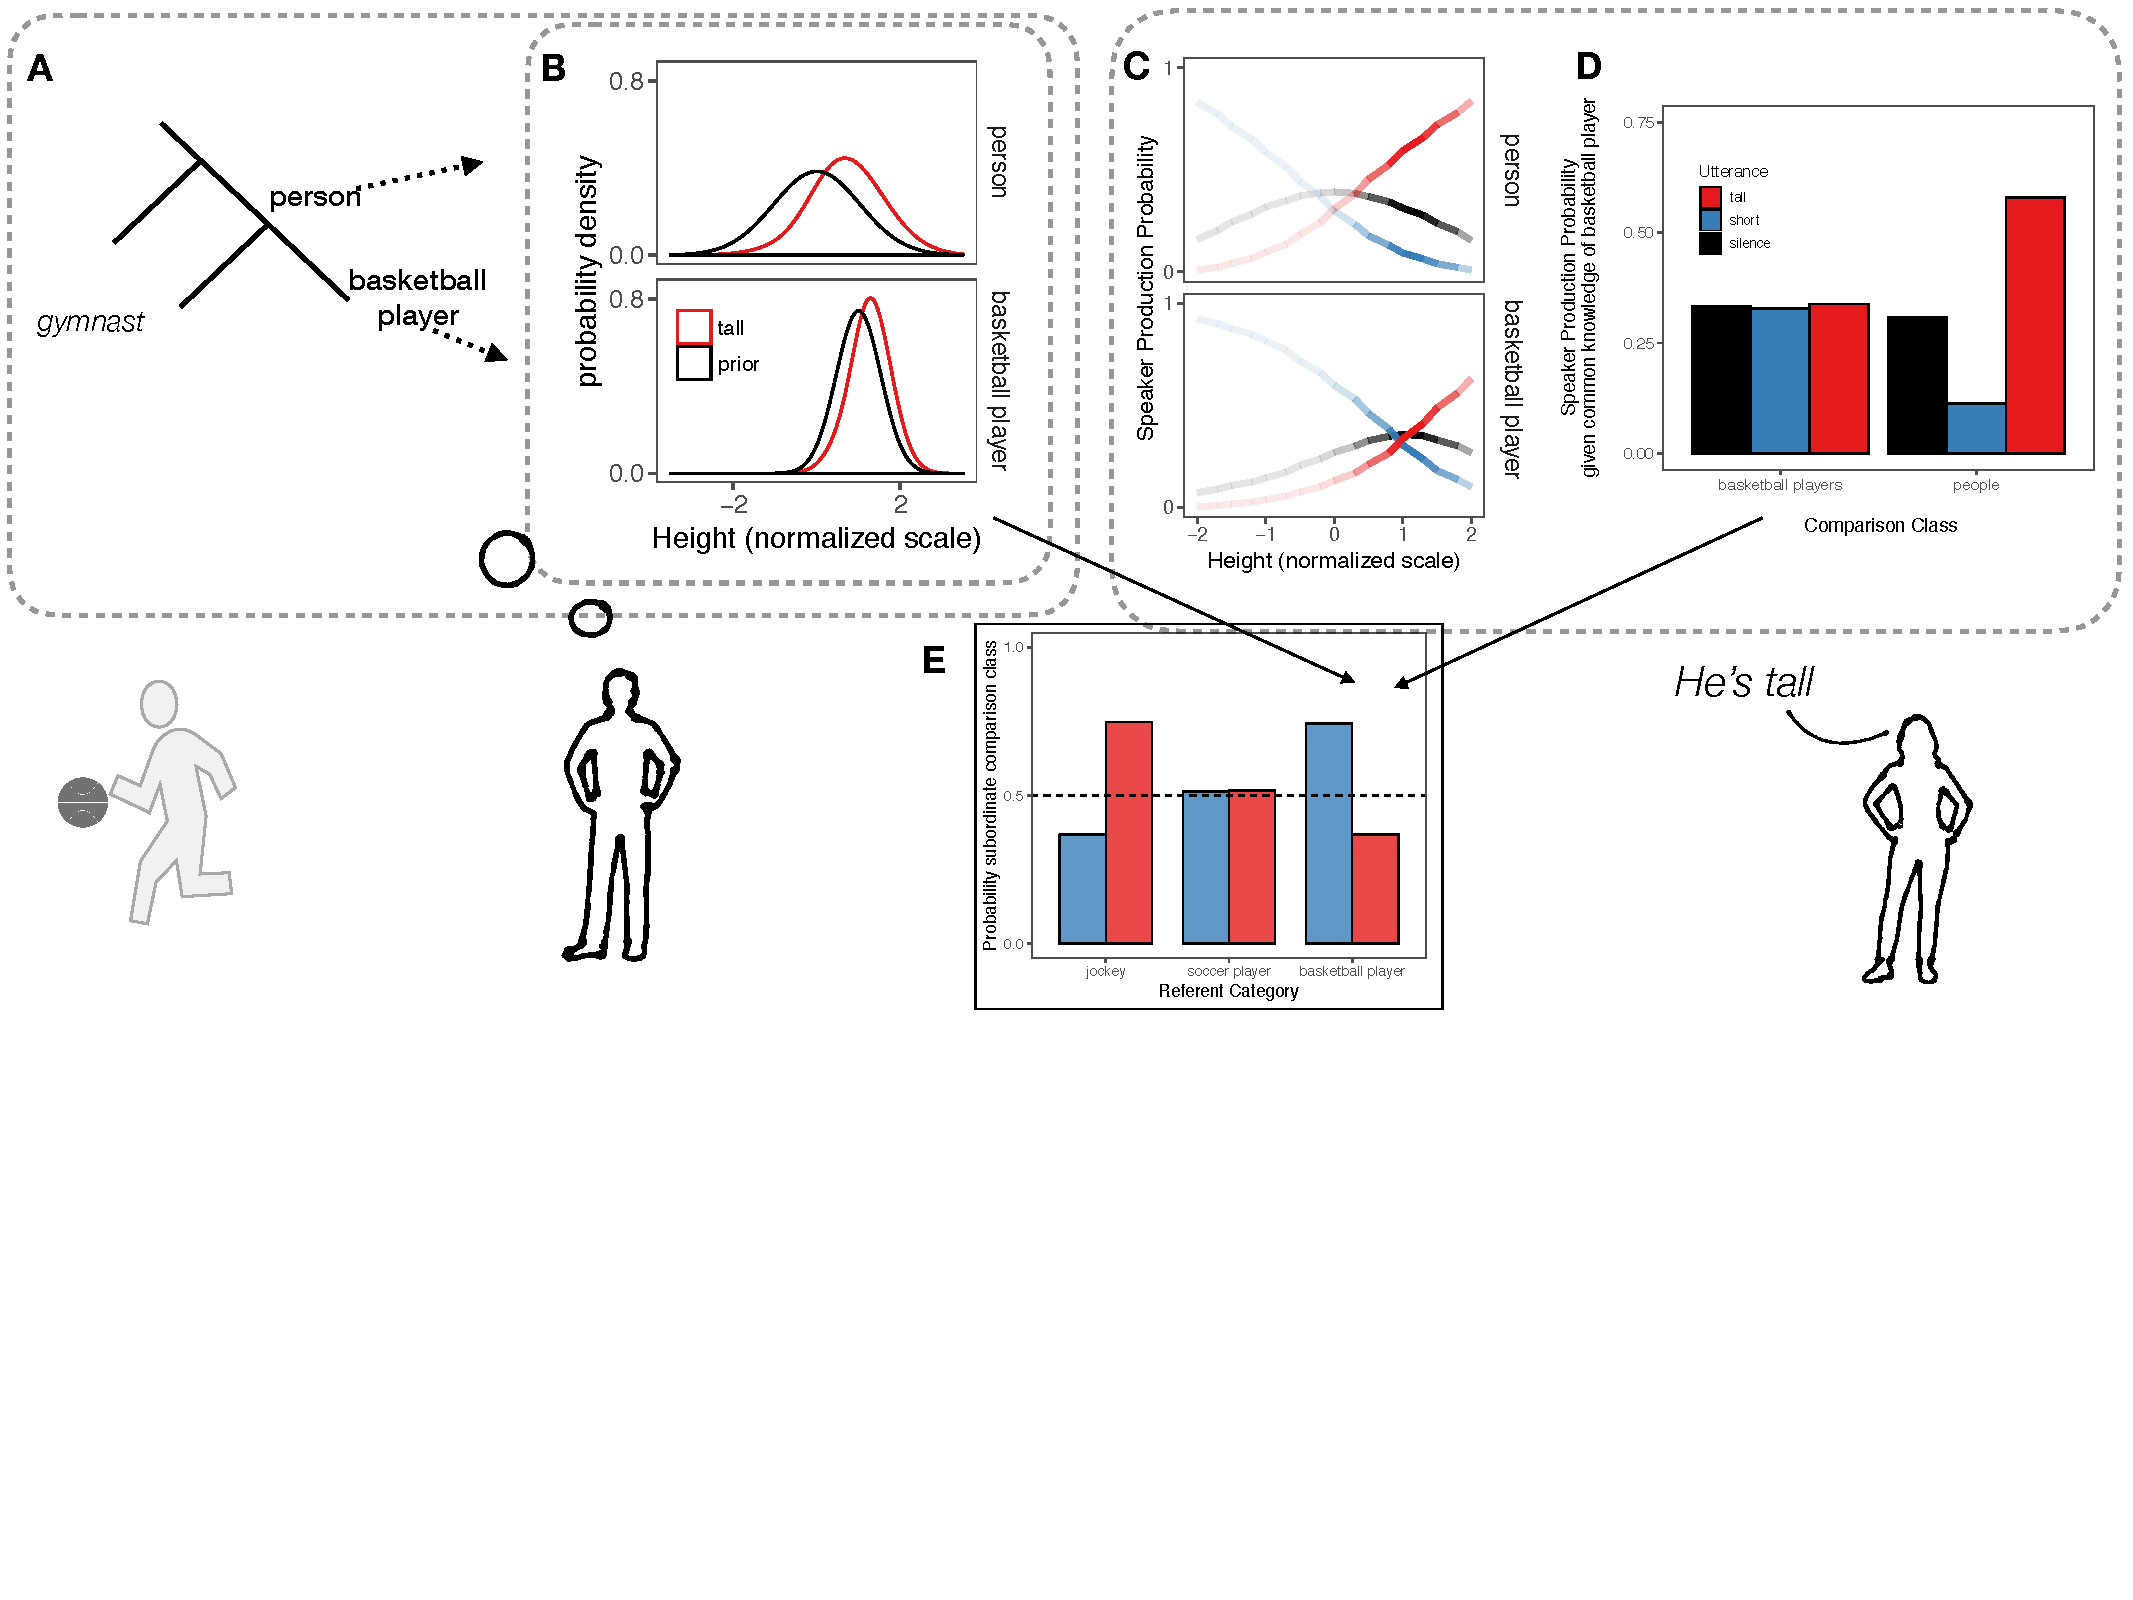
\includegraphics[width=\textwidth]{figs/model_cartoon.pdf}
\caption{\small \label{fig:modelCartoon}Model overview. A: A hypothesis space of comparison classes is constructed over a taxonomic hierarchy. B: A specific comparison class is realized as a probability distribution over the relevant degree (e.g., height; shown in black). The interpretation of a gradable adjective (e.g., \emph{tall}; shown in red)---given by $L_{0}(x \mid u, c)$---is sensitive to the comparison class. C: Listener $L_1$ imagines what a speaker $S_1$ would say given different comparison classes (facets) and assuming different possible heights of the referent (x-axis); the intensity of the colors (alpha/opacity) is in proportion to the listener's expectation of that particular height (e.g., the listener knows the referent is a basketball player, and so expects heights towards the upper range of the scale). D: Distribution of speaker utterances for different comparison classes marginalizing over the plausible heights of the referent. A speaker is more likely to say \emph{tall} is the comparison class is \emph{people}. E: Comparison class inference by the listener in terms of the probability of a subordinate class (e.g., basketball players) computed by inverting the speaker model. Listener is more likely to infer \emph{basketball players} as the comparison class when the referent is described as \emph{short} than when they are described as \emph{tall}.
% speaker production probability distributions are shown with the.
}
\end{figure}


\begin{align}
S_1(u \mid x, c) &\propto \exp{(\alpha \cdot (\ln L_{0}(x \mid u, c) - \text{cost}(u) ))}\label{eq:S1} 
\end{align}
%exp{(\alpha_1 \cdot \ln {L_{0}(x \mid u, \theta)} )}

We assume the speaker has three utterances she can say: \{\emph{tall}, \emph{short}, silence\}, where silence is a semantically vacuous utterance (i.e., a null action). 
The listener who updates their beliefs about the temperature given a vague adjectival utterance and a fixed comparison class $L_0(x \mid u, c)$ is model of context-sensitive adjective interpretation, a problem which has garnered a lot of recent attention by formal models of language understanding \cite{Lassiter2013, Qing2014a, Lassiter2017}.
We use a model of a literal listener which, following standard treatment in formal semantics \cite<e.g.,>{Kennedy2007}, takes the literal meaning of a gradable adjective to be simply a threshold function on the degree (e.g., \([\![tall]\!] = height > \theta\)) that gets combined with the listener's prior knowledge of the comparison class to produce a comparison class-specific interpretation of an adjective (Figure \ref{fig:modelCartoon}B).\footnote{Following standard treatment of antonyms, the
  semantics of \emph{short} are a threshold function on a distinct
  threshold variable: \([\![u_{short}]\!] = height < \theta_{short}\)), which
  is also inferred via the pragmatic listener (i.e., the listener infers
  a threshold for both \emph{tall} and \emph{short}). The pragmatic
  inferences about the comparison class that are the focus of this paper
  are invariant to whether or not the antonym is included in the
  alternative set. The comparison class inferences are also invariant to
  whether or not the antonym gets assigned its own unique threshold
  (\(\theta_{short}\)).}
  %
  \begin{align}
L_{0}(x, \theta \mid u, c) &\propto {\delta_{[\![u]\!](x, \theta)} \cdot P(x \mid c)} \cdot P(\theta) \label{eq:L0}\\
L_{0}(x \mid u, c) &= \int_{\theta} L_{0}(x, \theta \mid u, c) \diff\theta \label{eq:L0_marg} 
\end{align}
%
Equation \ref{eq:L0} is a model of literal listener who updates their prior beliefs about the degree given a comparison class $P(x\mid c)$ via a threshold function, represented by the Kronecker delta function \(\delta_{\mbox{ $[\![ u ]\!]$}(x, \theta)}\) that returns probabilities proportional to \(1\) when the utterance is true (i.e., when \(x > \theta\)) and \(0\) otherwise.
\citeA{Lassiter2013, Lassiter2017} showed how the context-sensitivity of gradable adjectives can be modeled as uncertainty about the threshold $P(\theta)$ (where $\theta$ comes from a uniform prior distribution over the support of the degree prior), which we adopt here in our literal listener model. 
Finally, we assume the communicative goal of using an adjective like \emph{tall} is to convey information about the height of the referent $x$; thus, the speaker model $S_1$ (Equation \ref{eq:S1}) chooses utterances to convey the height $x$ to the literal listener $L_0$, which we calculate by marginalizing out the threshold variable $\theta$ (Equation \ref{eq:L0_marg}).
%Our model of comparison class inference builds on top of these formal theories, and we treat this model component $L_{0}(x \mid u, c)$ as a black-box function that produces a probability distribution over degrees (e.g., heights) in a manner that is sensitive to the comparison class (e.g., respecting the interpretative difference between \emph{tall person} and \emph{tall basketball player}; ). 
%\red{Figure 1 shows the behavior of this model component.}
%We adopt the model of \citeA{Lassiter2013, Lassiter2017}   A full presentation of this  part of the model is given in Appendix A.
  
\subsection{Model behavior}

We consider an idealized case where the comparison class can be either a relatively specific (e.g., subordinate-level, \(c_{sub}\)) or relatively general (e.g., basic-level, \(c_{basic}\)) categorization (e.g., tall relative to \emph{basketball players} or relative to \emph{people}): \(c \in \{c_{sub}, c_{basic}\}\).
To understand the model behavior, consider the speaker model \(S_1\) under different assumptions (by the listener) about the implicit comparison class: \(S_{1}(u \mid x, c = c_{sub})\) and \(S_{1}(u \mid x, c = c_{basic})\). 
Figure \ref{fig:modelCartoon}C shows the speaker production probabilities of the three possible utterances for each value along the degree scale (e.g., each height) for the two different comparison classes.  If the comparison class is \emph{people}, the speaker will produce \emph{tall} when the height of the referent is substantially greater than the average height for people, with the speaker more likely to say \emph{tall} as the height of the referent increases.
  If the comparison class is \emph{basketball players}, the speaker's criterion shifts to the right and she becomes more reluctant to produce \emph{tall} until the height of the referent is much greater. 
  The listener combines this generative model of adjectival utterances with his prior knowledge about the height of the referent: The listener knows the referent is a basketball player and thus their height is sampled from the basketball player distribution (Figure \ref{fig:modelCartoon}B, bottom, black; this distribution is superimposed as an opacity on Figure \ref{fig:modelCartoon}C).
  When the listener marginalizes over their beliefs about the height of the referent, the speaker is more likely to produce \emph{tall} if the comparison class were \emph{people} (Figure \ref{fig:modelCartoon}D).  

The listener inverts this generative model of the utterance (i.e., the speaker model) to infer the implicit comparison class (Figure \ref{fig:modelCartoon}E).
Because the speaker is more likely to stay \emph{tall} if the comparison class were \emph{people}, the listener reasons that a speaker who says \emph{tall} probably was assuming a more general comparison class (i.e., that the comparison class is \emph{people}). 
If, however, the listener hears of the basketball player that he is \emph{short}, the more likely comparison class is the subordinate class of \emph{basketball players}.
This inference is driven by prior knowledge about the category, and thus, we would expect the inferences to change if the prior knowledge changes.
Indeed, the same adjectives used to describe a member of a subordinate category that tends to fall low on the degree scale (e.g., jockeys, who tend to short people) will result in the opposite inferences about the comparison class. 
Thus, our model predicts that the comparison class can be flexibly adjusted and it provides a precise quantitative formulation in how this inference should be driven. 

\begin{figure}
\centering
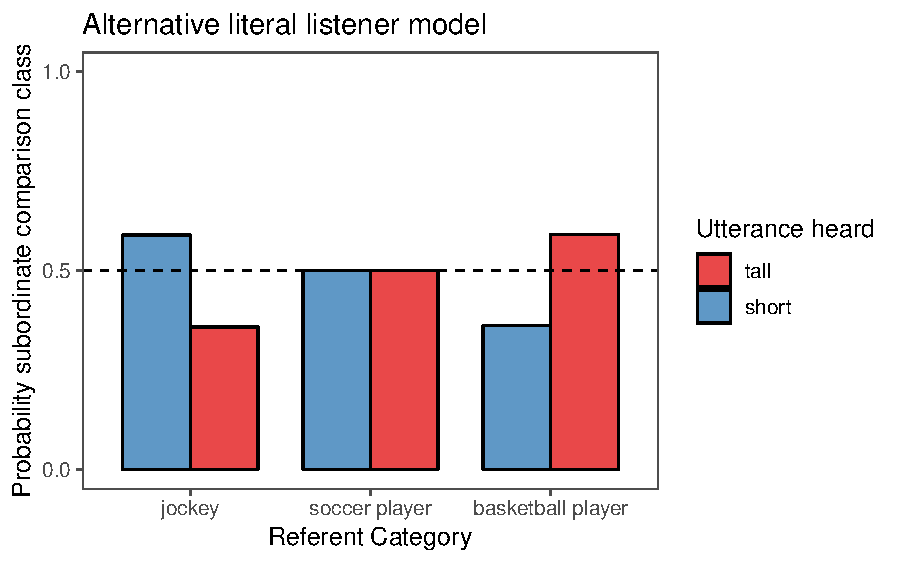
\includegraphics[width=0.6\textwidth]{figs/cc_inference_L0.pdf}
\caption{\small \label{fig:alternativeModelPredictions}Alternative model predictions for a literal model that does not represent a speaker's representation of the context as separate from their own. This listener effectively answers the question of what is more likely: a basketball player who is tall or a person who is tall?
% speaker production probability distributions are shown with the.
}
\end{figure}

\subsection{Alternative model}

The inference about the comparison class is necessarily a pragmatic inference involving representing a speaker's beliefs about the context separately from the listener's beliefs about the context. 
This can be seen by comparing Equations \ref{eq:L1} and \ref{eq:L0}: the pragmatic listener $L_1$ uses a prior distribution over the degree given their knowledge of the referent $P(x \mid k)$ whereas the literal listener $L_0$ uses a distribution conditional on the comparison class $P(x \mid c)$. 
This separation of the listener's knowledge of the referent $k$ from the comparison class $c$ is necessary for the comparison class inferences shown in Figure \ref{fig:modelCartoon}E.
A purely Bayesian listener model, who has uncertainty about the comparison class as well as all of the other parameters of the full model (the degree $x$ and the threshold $\theta$), but does not separate their knowledge of the referent from the speaker's representation of the context is given by: 
%
  \begin{align}
L_{0}(x, \theta, c \mid u, k) &\propto \delta_{[\![u]\!](x, \theta)} \cdot P(x \mid c) \cdot P(c \mid k) \cdot P(\theta) \label{eq:L0alt}
\end{align}
%
This listener uses their knowledge of the referent $k$ to constrain only the hypothesis space of comparison classes but not to separate the speaker's representation of the context from their own. 
In effect, this listener is answering a different question, a question more about the referent than the comparison class: what is more likely---a basketball player whose height is greater than some threshold or a person whose height is greater than some threshold? This literal listener model predicts the exact opposite pattern of results from the pragmatic listener model (Figure \ref{fig:alternativeModelPredictions}). 
%The utterance which does not reference a class (e.g., It's warm}) inherits the same meaning as the utterance with the explicit class that
%matches the assumed implicit class (i.e., if \(c_{i} = c_{sub}\), then
%\(u_i\) has the same meaning as \(u_{sub}\)). Therefore, reasoning about
%the likely comparison class reduces to reasoning about which explicit
%utterance the speaker would have been more likely to say.
  


\section{Overview of Experiments}

\begin{figure*}[htb]
{\centering 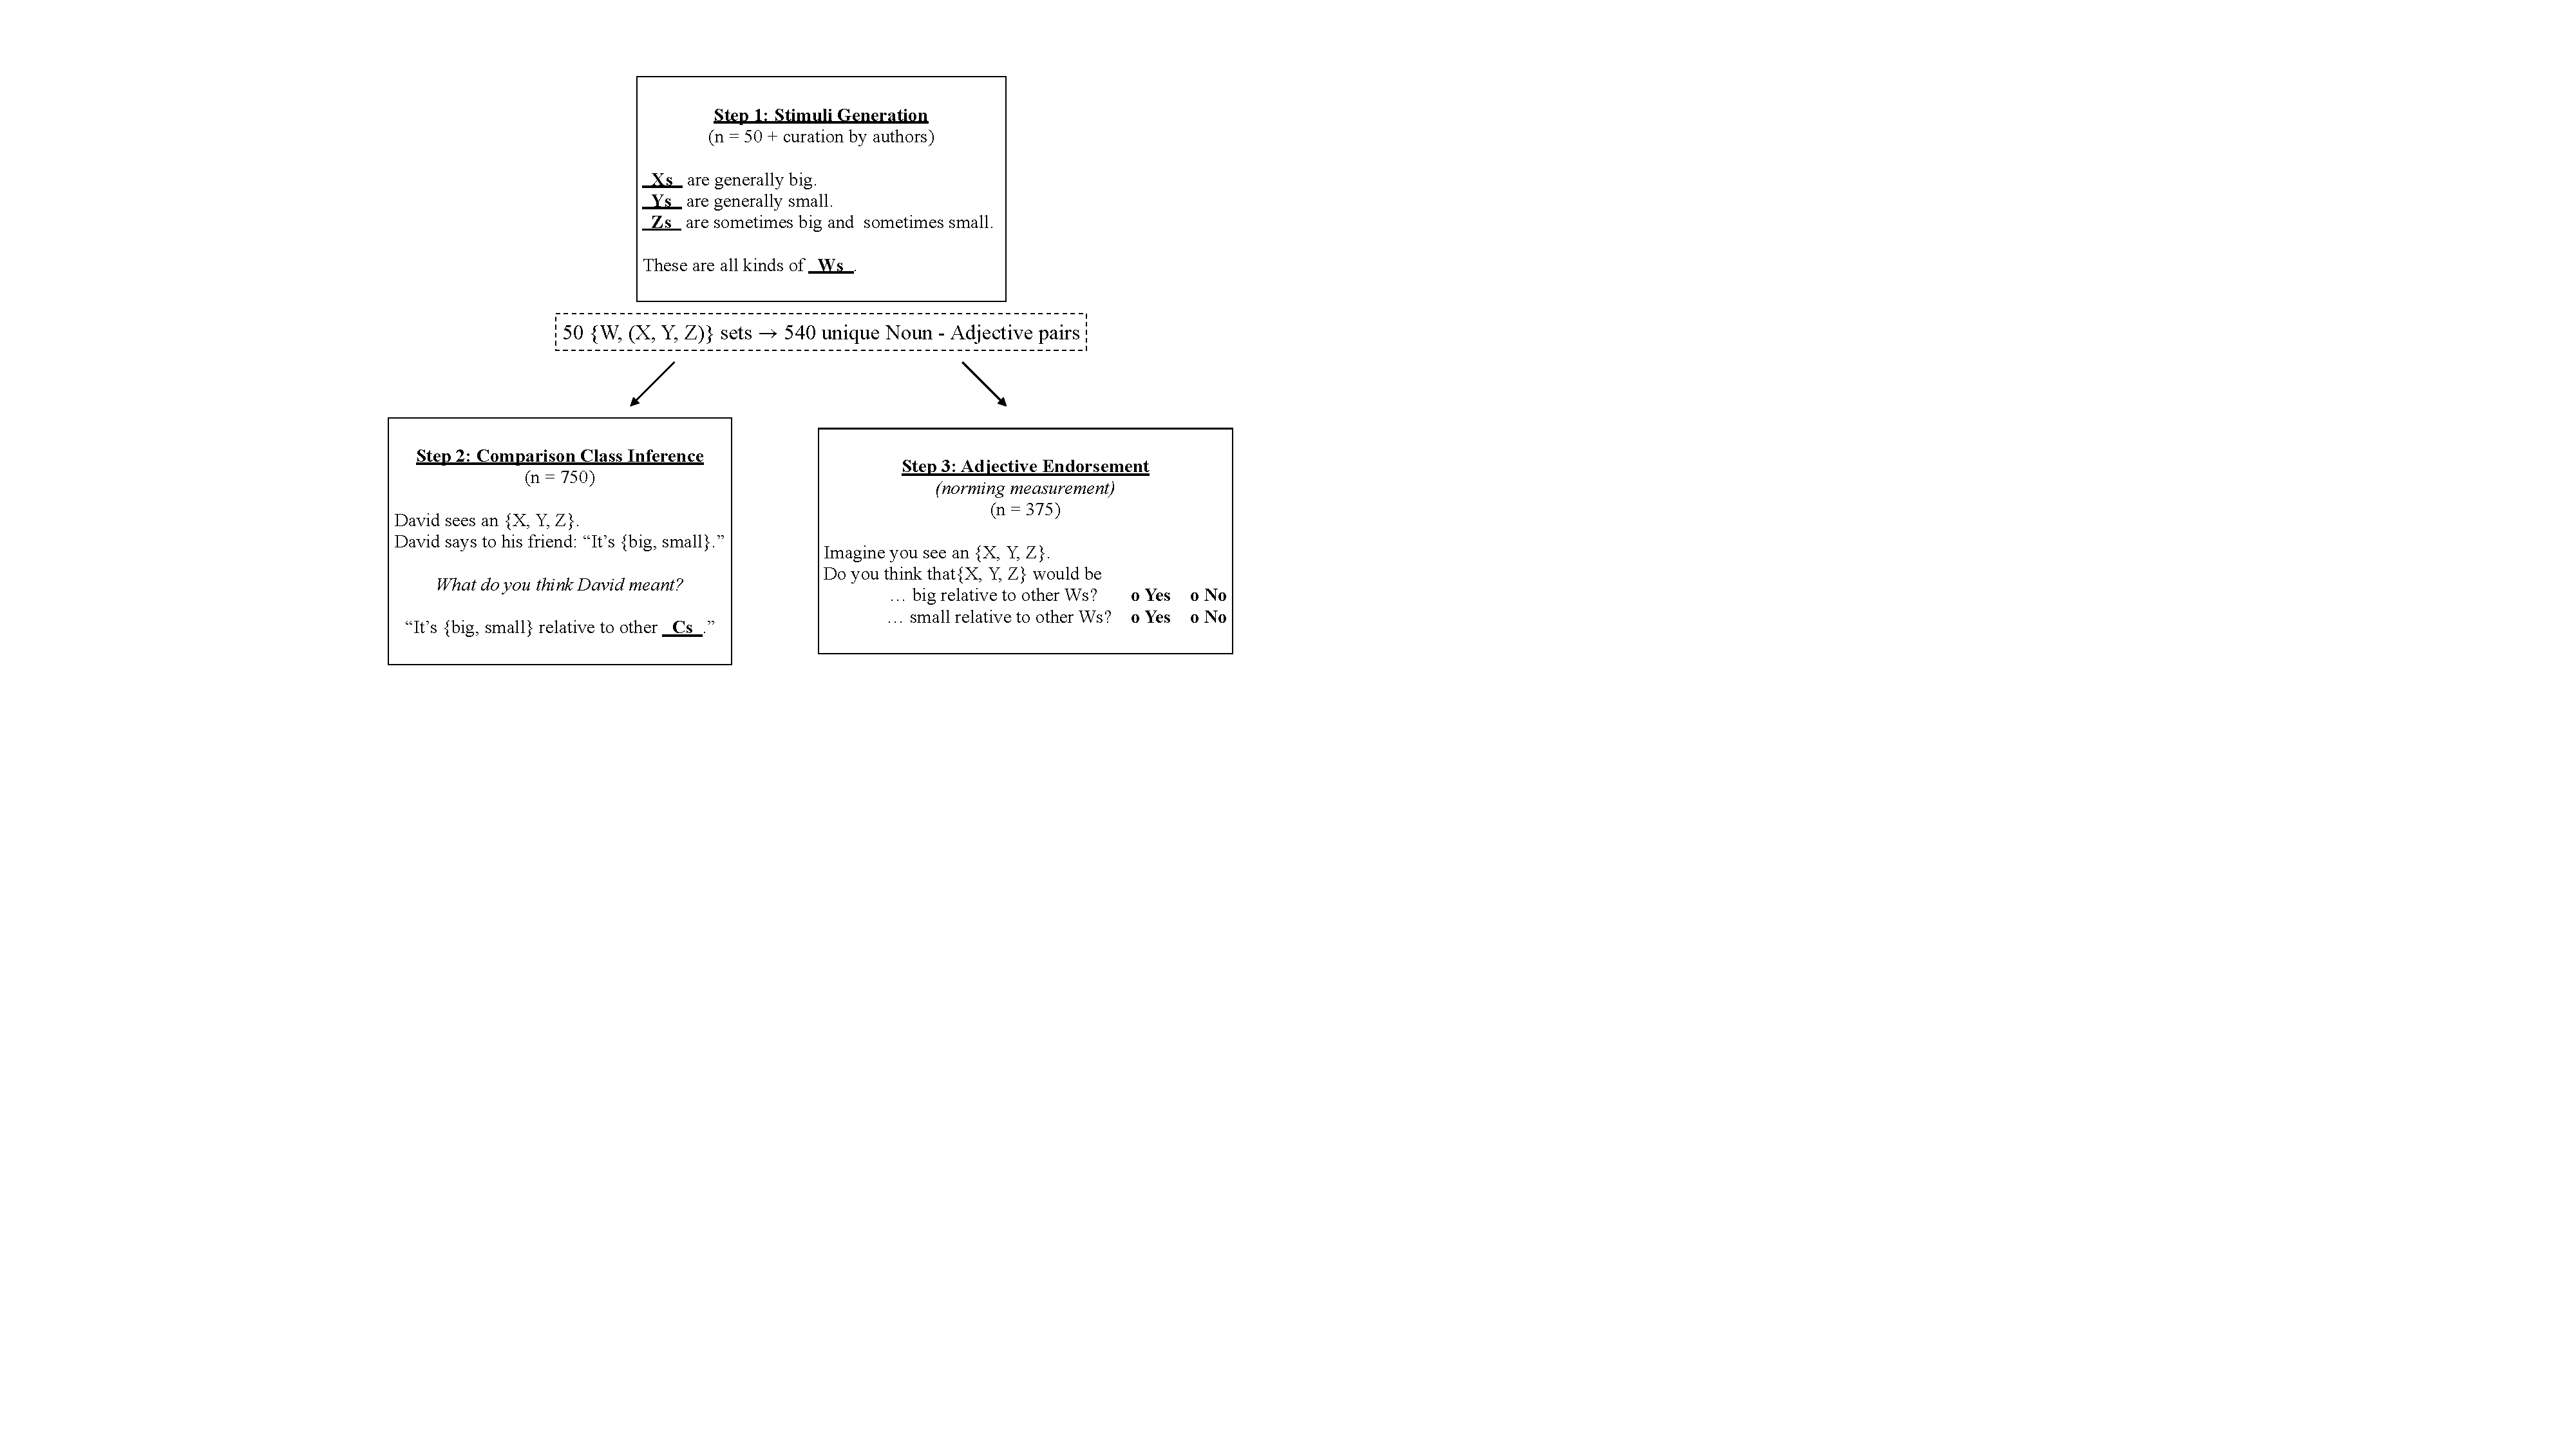
\includegraphics[width=1\textwidth]{figs/expt_overview} }
\caption{\small Overview of Experiments. Step 1: Using a structured production task, we elicit sets of stimuli that all share the feature of containing categories generally judged as having either a positive or negative adjective  (\emph{X, Y}; e.g., big or small) applied to them as well as a control category (\emph{Z}; e.g., sometimes big and sometimes small). The task is designed in a way to elicit three categories of the same basic- or superordinate-level category (\emph{W}). Step 2: Forced-choice task where participants judge whether a member of the subordinate level category would be judged as a having the adjective applied explicitly relative to the basic/superordinate level category. This task serves to validate our experimental stimuli as well as provide additional data to constrain the parameters of the comparison class inference model. Step 3: Free-production task to elicit the comparison class.}\label{fig:exptOverview}
\end{figure*}

We test our hypothesis that the comparison class can be flexibly adjusted based on world knowledge and pragmatic principles in a set of coordinated experiments (Figure \ref{fig:exptOverview}).
We first empirically elicit test stimuli by having participants fill out phrasal templates that aim to elicit sets of categories at the same level of abstraction, which differ in general expectations (e.g., categories whose members are generally big, generally small, or sometimes big and sometimes small; Experiment~1). 
From this set, we curate a set of experimental stimuli which we use in the following experiments.
Experiment 2 is the main comparison class inference experiment, in which participants rephrase a speaker's statement in a way that makes the comparison class explicit.
Experiment 3 is an adjective endorsement (or, truth judgment) task which uses the same categories that were used in Experiment 2.
In this task, participants are asked to judge whether an adjective (e.g., \emph{big} or \emph{small}) would be true of a member of a subordinate category relative to the basic or superordinate category. 
This task provides additional data to constrain the parameters of the comparison class inference model (described below).
The quantitative predictions of the model are tested using a Bayesian data analytic strategy, where we explicitly model the data from both the Comparison Class Inference (Experiment~2) and Adjective Endorsement (Experiment~3) tasks.
This joint Bayesian data-analytic strategy allows us to infer, rather than stipulate, the world knowledge that guides the inference about the comparison class in the computational model. 
%\mht{may want to reverse the order, if we use the modal superordinate comparison class from the Inference experiment as the comparison class in the Adjective Endorsement experiment}

\section{Data-analytic Strategy}

Our comparison class inference model makes qualitative predictions about the likely comparison class assumed by a speaker when they hear a scalar adjective (e.g., \emph{he's tall}; Figure \ref{fig:modelCartoon}E). 
The model is quantitative in nature, however, and can make quantitative predictions concerning the strength of comparison class inferences given model parameters that describe world knowledge $P(x)$ and prior expectations about the comparison class $P(c)$.

Previous modeling papers in the RSA tradition empirically elicit world knowledge $P(x)$ through prior elicitation tasks.
These tasks often involve estimating numerical quantities or making probability judgments, for which the participant must have relevant knowledge concerning the units of measure (e.g., prices in dollars) and for which complicated linking functions are often designed to relate latent probabilities to the estimation data \cite{Franke2016}. 
We take a different approach: We make small modifications to the same core RSA architecture to make predictions about a related language task concerning the same domains used in the Comparison Class Inference task. 
We then construct a Bayesian data analytic model to infer the world knowledge shared between these two tasks, along with the few other free parameters of the full BDA-RSA model (Figure \ref{fig:bayesnet}). 
This \emph{descriptive Bayesian approach} \cite{tauber2017} coupled with explicit models of language understanding allow us to model broader coverage data sets while still constraining model flexibility because the models must predict more distinct data points. 

In our model, world knowledge is represented by probability distributions over degrees (e.g., heights).
Comparing interpretations of the same adjective across different comparison classes is an inherently relative judgment; thus, only the relative values for the degrees affect model predictions. 
Hence, we fix each general (basic/superordinate) class in each domain to be a standard normal distribution---$P(x \mid c = c_{basic}) = \mathcal{N}(0, 1)$---and assume the specific (subordinate/basic) priors to also be Gaussian distributions---\(P(x \mid c = c_{sub}) = \mathcal{N}(\mu_{sub}, \sigma_{sub})\); the subordinate priors thus have standardized units.
These parameters vary by the category $k = c_{sub}$ as well as the degree scale (e.g., height vs. weight).
We infer the plausible values of the parameters governing the subordinate priors from the data.

The data from the comparison class experiment would be insufficient, however, to reliably estimate the model parameters governing the world knowledge priors. 
To alleviate this, we use the same RSA architecture to predict additional data about the related Adjective Endorsement task. 
In the Adjective Endorsement task, participants are asked to judge whether a gradable adjective (e.g., \emph{big} or \emph{small}) would be true of a member of a subordinate-level category relative to the basic- or superordinate level category (e.g., \emph{Do you think that they  [a basketball player] would be tall relative to other people?}).
To model the adjective endorsement data, we remove comparison class uncertainty from the model (since the task provides the comparison class explicitly) and, following \citeA{Tessler2019psychrev}, model sentence endorsement as a speaker deciding whether or not to produce the adjectival utterance to the listener: $S_{1}(u \mid k) \propto \exp{(\alpha_2 \cdot {\mathbb E}_{x\sim P_{k}}} \ln{L_0(x \mid u)})$, where $L_0(x \mid u)$ is given by Eq. \ref{eq:L0}. 

The prior distribution over comparison classes $P(c \mid k)$ reflects listeners' expectations of what classes are likely to be discussed, given that the referent is a member of a particular subordinate category $k$.
We simplify the full comparison class inference problem to deal with reasoning about only a specific~vs.~general class.
This prior probability of these comparison class plausibly includes a basic-level bias \cite{rosch1975family} but could also reflect how frequently these classes are used in conversation.
We estimate frequency from the Google WebGram corpus $\hat{f}_k$ and combine it wit
We model comparison class usage frequency as a logistic function with an intercept and slope: $P(c) \propto \beta_0 + \beta_1 \cdot \log (\hat{f}_k)$

%The RSA listener (Eq. \ref{eq:L1a}) and speaker (Eq. \ref{eq:S2}) models make quantitative predictions about comparison class interpretation and adjective endorsement, respectively.
We construct a single data-analytic model with each of these RSA components as sub-models in order to make quantitative predictions about the data from both of our experiments.
The listener and speaker sub-models share their prior world knowledge $P(x \mid k)$ (e.g., heights of basketball players).
We put the same priors over the parameters of each subordinate distribution $k$ for each degree $k$: $\mu^d_k \sim \text{Uniform}(-3, 3)$, $\sigma^d_k \sim \text{Uniform}(0, 5)$, since they have standardized units.
The comparison class prior $P(c \mid k)$ scales the empirical frequency $\hat{f}_k$ by a free parameter, which we give the following prior: $\beta \sim \text{Uniform}(0, 3)$. 
Each RSA model has an additional speaker optimality parameter $\alpha_{i}$ not of direct theoretical interest.
We use priors consistent with the previous literature: $\alpha_i \sim \text{Uniform}(0, 20)$.
We implemented the RSA and Bayesian data analysis models in the probabilistic programming language WebPPL \cite{dippl}.

%The comparison class inference model has one speaker optimality: $\alpha^\text{1}_{1}$.
%The adjective endorsement model has two speaker optimality parameters: 
%$\{\alpha^\text{2}_{1}, \alpha^\text{2}_{2}\}$.


\begin{figure}[ht!]
  \begin{center}
    \begin{tabular}{cc}
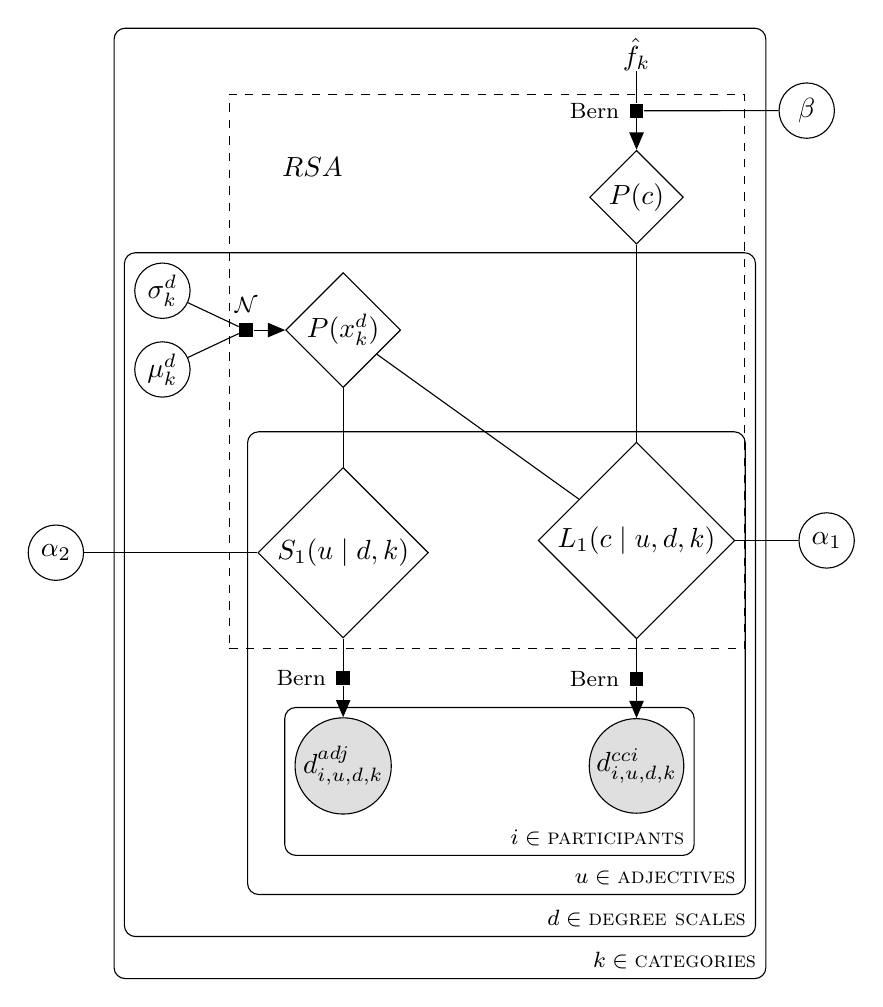
\begin{tikzpicture}


  % Y
  \node[obs]          (d-c)   {$d^{cci}_{i, u, d, k}$}; %
  \node[obs, left=2.5 of d-c]          (d-a)   {$d^{adj}_{i, u, d, k}$}; %
  \factor[above=of d-a] {da-f} {left:Bern} {} {} ; %
  \factor[above=of d-c] {dc-f} {left:Bern} {} {} ; %

  \node[det, above=of d-c] (L1) {$L_1(c \mid u, d, k)$} ; % 
  \node[det, above=of d-a] (S2) {$S_1(u \mid d, k)$} ; % 
  
  \node[det, above=of S2]  (x)   {$P(x^d_k)$}; %
  \node[det, above=2.5 of L1] (c)   {$P(c)$}; %

   \node[const,  above=1 of c] (fhat) {$\hat{f}_k$} ; %
%   \node[const, right=1.3 of c, yshift=1.5cm] (fshat) {$\hat{f}_s$} ; %
   \node[latent, right=1.2 of c, yshift=1.1cm]  (b) {$\beta$} ; %
   \factor[above=of c] {c-f} {left:Bern} {fhat,b} {c} ; %

  \node[latent, left=1.2 of x, yshift=-0.5cm] (mx) {$\mu^d_k$} ; %
  \node[latent, left=1.2 of x, yshift=0.5cm]  (sx) {$\sigma^d_k$} ; %
  \factor[left=of x] {x-f} {above:$\mathcal{N}$} {mx,sx} {x} ; %

  % sopt
   \node[latent, right=0.8cm of L1, yshift=0.0cm]         (a1)   {$\alpha_1$}; %
   \node[latent, left=2.2cm of S2]         (aa1)   {$\alpha_2$}; %
%   \node[latent, left=2.5cm of S2, yshift=-0.6cm]         (aa2)   {$\alpha^{adj}_2$}; %
 % \node[const, above=of t, xshift=-0.5cm] (at)  {$\alpha_\tau$} ; %
  % \node[const, above=of t, xshift=0.5cm]  (bt)  {$\beta_\tau$} ; %

  % Factors
%  \factor[above=of t] {t-f} {left:$\mathcal{G}$} {at,bt} {t} ; %
\factoredge {L1} {dc-f} {d-c} ; %
\factoredge {S2} {da-f} {d-a} ; %
%\factor       {W'-f}   {Multi} {} {};  %
  % Connect w and x to the dot node
  \edge[-] {c,x} {L1} ;
  \edge[-] {x} {S2} ;
%  \edge[-] {L1} {RSA} ;
%  \edge[-] {S2} {RSA} ;
  \edge[-] {a1} {L1} ;
%  \edge[-] {a1} {S2} ;
  \edge[-] {aa1} {S2} ;
%  \edge[-] {aa2} {S2} ;

\gate {RSAgate} {(L1)(S2)(x)(c)(x-f)(c-f)} {} ; %
\node[text width=1cm] at (-4,7.6) {$RSA$};
  % Plates
    \plate {dataPlate} {
     (d-c)(d-a)
  } {$i \in \textsc{participants}$} ;
  
  \plate {adjPlate} { %
    (dataPlate)
     (S2) (L1) 
  } {$u \in  \textsc{adjectives}$} ;
  
        \plate {degreePlate} { %
 (adjPlate)    (dataPlate)
  (x)(x-f)(mx)(sx)
  } {$d \in  \textsc{degree scales}$} ;
  
  \plate {subPlate} { %
  (adjPlate)    (dataPlate)(degreePlate)
   (fhat) (c-f) (c)%
    %(RSA) 
    (S2) (L1) (RSAgate)%%
  } {$k \in  \textsc{categories}$} ;
%    \plate {superPlate} { %
%(adjPlate)  (subPlate)(fshat)    (dataPlate)(degreePlate)
%  } {$s \in  \textsc{superordinate categories}$} ;

    
%  \plate {} {%
%    (d-c)(dc-f)(dc-f-caption) %
%    (c)(da-f)(da-f-caption) %
%    (RSA) %
%    (yx.north west)(yx.south west) %
%  } {$M$} ;




%  % Define nodes
%  \node[latent]                             (u) {$u$};
%  \node[latent, above=of u, xshift=-1.2cm] (c) {${c}$};
%  \node[latent, above=of u, xshift=1.2cm]  (x) {${x}$};
%  \node[latent, above=of c, xshift=0cm] (f) {${f}$};
%  \node[latent, above=of x, xshift=0cm] (g) {${g}$};
%
%  % Connect the nodes
%  \edge {c,x} {u} ; %
%  \edge {f} {c} ; %
%  \edge {f,g} {x} ; %


\end{tikzpicture}

    \end{tabular}
  \end{center}
  \caption{\small Joint Bayesian data analytic strategy to infer model parameters and generate model predictions. Two similar RSA models (an adjective endorsement model $S_1$ and the comparison class inference model $L_1$) directly predict the data from Experiments 2 \& 3 ($d^{adj}$ and $d^{cci}$), respectively. Each of these models relies upon world knowledge $P(x^d_k)$ (e.g., prior expectations about the height of a basketball player), which are assumed to be Normal distributions with unknown mean $\mu^d_k$ and variance $\sigma^d_k$), that vary by category (basketball player) and degree (height). The prior on comparison classes $P(c \mid k)$ varies according to the subordinate and superordinate categories, is used only in the $L_1$ model, and is assumed to be a linear function of the log frequency of the noun phrase $\hat{f}_k$, with global scale parameter $\beta$. Each RSA model has its own speaker optimality parameter $\alpha$.}
  \label{fig:bayesnet}
\end{figure}





%To match the  we code the behavioral responses as to whether or not the mention the subordinate level category that is used to describe the referent in the experimental context. 
%
%
%Inferring the comparison class is necessarily a problem of inferring the intentions of another person.
%The relevant question is not \emph{is today a day in winter?} (an inference about the world), but rather \emph{did the speaker mean to draw a comparison to days to winter?} (an inference about intentions).
%Thus, a model for comparison class inference necessarily involves social reasoning about the speaker's intentions.
%
%Thus, the listener's beliefs about the temperature is a probability distribution conditional on the speaker and listener shared beliefs as well as the listener's private beliefs: $P(x \mid f, g)$.
%In the contexts we consider, the listener has no private beliefs and the totality of relevant shared beliefs boils down to the most specific categorization that the listener believes to be true of the referent (i.e., the day is a day in winter).

%On the other hand, on the shared beliefs $g$ can be used to guide 

%
%Both sets of beliefs can constrain the listener's belief distribution over the relevant degree as applied to the referent: If the listener knows that the day is a day in winter, they should use that information to guide their knowledge about the likely value of the degree $P(x \mid f, g)$.
%
%
%We model the scenario where a listener hears a gradable adjective describing a referent (e.g., that the temperature outside is warm) but does not know the comparison class assumed by the speaker. 
%To do this, a listener draws on their knowledge of the referent (e.g., that the day is a day in winter)
%
%When understanding vague language like a gradable adjective in context, a listener must integrate what they know about 
%
%Thus, we begin with a model for gradable adjective interpretation and build a mechanism for comparison class inference on top of this model. 
%. Where does this comparison class come from?
%
%We hypothesize that listeners maintain uncertainty about multiple
%possible comparison classes, but can reduce their uncertainty by
%combining world knowledge with pragmatic reasoning. More specifically,
%listeners use their world knowledge of what worlds are plausible under
%different comparison classes \(P(x \mid c)\) (e.g., the likelihood of
%different temperatures within different seasons), what implicit
%comparison classes are likely to be talked about \emph{a priori}
%\(P(c_i)\) (\(i\) for implicit), and how a rational speaker would behave
%in a given world assuming a particular comparison class
%\(S_{1}(u \mid x, c_i, \theta)\) (Eq. \ref{eq:L1a}). 
%
% As in previous models, we
%assume the listener is aware that the referent is a member of the
%subordinate class (and by extension, the superordinate as well). We
%additionally assume the pragmatic listener uses the most subordinate
%class information to inform the likely values of the degree (e.g., the
%listener's prior over temperatures is given by the distribution of
%temperatures for a specific class such as \emph{winter}
%\(P(x \mid c = c_{sub})\)). With these assumptions, the model becomes:
%
%\begin{align}
%L_{1}(x, c_{i}, \theta \mid u) &\propto S_{1}(u \mid x, c, \theta) \cdot P(x \mid c =  c_{sub}) \cdot P(c_{i}) \cdot P(\theta) \label{eq:L1a}\\
%S_{1}(u \mid x, c_i, \theta) &\propto \exp{(\alpha_1 \cdot \ln {L_{0}(x \mid u, c_i, \theta)}- \text{cost}(u)) } \label{eq:S1a}\\
%L_{0}(x \mid u, c_i, \theta) &\propto {\delta_{[\![u]\!](x, \theta)} \cdot P(x \mid \text{parseClass}(u, c_i))} \label{eq:L0a}
%\end{align}
%
%We are interested in the behavior of the pragmatic listener model with
%he hears an utterance without an explicit comparison class \(u_{i}\)
%(e.g., ``It's warm''). The listener reasons about alternative
%utterances the speaker could have said in order to draw pragmatic
%inferences. In this model, we assume the speaker has the option of
%conveying the adjective with an explicit comparison class \(u_{sub}\)
%and \(u_{super}\) (e.g., ``It's warm relative to other days in
%winter'' and ``It's warm relative to other days of the year'').
%The literal meanings of these alternatives are the same as the
%underspecified utterance (i.e., a threshold function:
%\([\![u_{warm}]\!] = x > \theta\)), but have the additional feature of
%overriding the implicit comparison class \(c_i\)and forcing the literal
%listener into a particular comparison class encoded in the utterance via
%the function \(\text{parseClass}\). That is:
%
%\begin{eqnarray}
%\text{parseClass}(u, c_i) & = &
%\begin{cases}
%c_{i} & \text{if } u = u_{i}\\
%c_{sub} & \text{if } u = u_{sub}\\
%c_{super} & \text{if } u = u_{super}\\
%\end{cases}
%\end{eqnarray}
%
%Thus, the speaker conditioning on a particular value for \(c_{i}\) only
%has implications for the literal listener if the speaker chooses to
%produce the implicit utterance (e.g., ``It's warm''). Should the
%speaker instead choose an utterance that explicitly articulates the
%comparison class (e.g., ``It's warm for winter''), the literal
%listener will use the explicit class to set his prior expectations
%\(P(x \mid c)\) via the \(\text{parseClass}\) operator.
%




%\subsubsection{Qualitative model predictions}


%\begin{figure*}[htb]

%{\centering 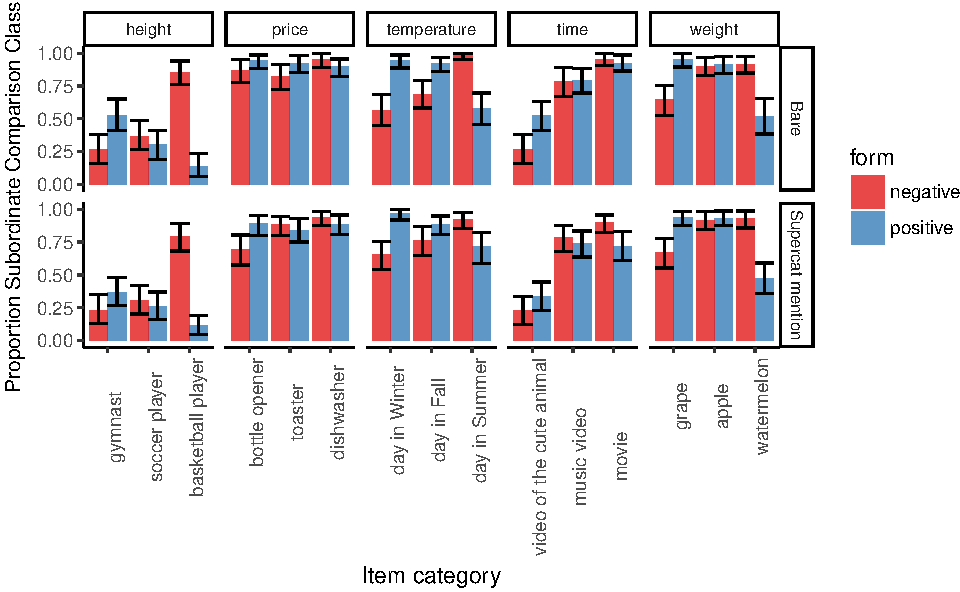
\includegraphics[width=1\textwidth]{figs/expt1results-1} 
%
%}
%
%\caption{Empirical comparison class judgments in terms of proportion in favor of subordinate comparison class.  Error bars correspond to 95\% Bayesian credible intervals.}\label{fig:expt1results}
%\end{figure*}
%
%\begin{figure*}[htb]
%
%{\centering \includegraphics[width=1\textwidth]{figs/modelParameters-1} 
%
%}

%\caption{Reconstructed degree priors (top) and empirically derived comparison class priors (botton). Top: Inferred prior distributions of world knowledge used to model Experiment 1 and 2 data. Bottom: Inferred prior probability of the subordinate comparison classes based on Google WebGram frequencies. Error bars correspond to 95\% Bayesian credible intervals, derived from the posterior on the $\beta$ scale parameter.}\label{fig:modelParameters}
%\end{figure*}

\section{Behavioral experiments}

We conduct three experiments to collect the data necessary to test the quantitative and quantitative predictions of our model, as outlined in Figure \ref{fig:exptOverview}. 

\subsection{Experiment 1: Stimuli Generation}

\subsubsection{Participants}

We recruited 50 participants from Amazon's Mechanical
Turk, restricted to those with U.S. IP addresses with at least a
95\% work approval rating. The experiment took about 5 minutes and
participants were compensated \$0.60 for their work.

\subsubsection{Materials}

We used 15 pairs of positive- and negative-form gradable adjectives that describe physical dimensions (Table \ref{tab:1}).
Some of the adjective pairs described the same dimension and/or had an adjective in common with another pair (e.g., \emph{fast}--\emph{slow} and \emph{quick}--\emph{slow}); these were included because we believed they would bring to mind different kinds of categories.

\subsubsection{Procedure}

On each trial, participants were given a phrasal template, for which they were asked to fill-in missing parts.
Three sentences in the template were missing subjects that were described as generally having the adjective apply to them (Figure \ref{fig:exptOverview}, Step 1). 
These sentences were followed with another that read that the three kinds of subjects from the previous sentences were ``all kinds of \_\_\_''.
This last sentence was introduced to constrain the kinds of responses to the first three sentences such that the subjects would be all members of the same basic- or superordinate level category. 

A template for ``big'' and ``small'' would look like: 
\begin{description}[noitemsep]
%\tightlist
\item \_\_\_\_\_ are generally big.
\item  \_\_\_\_\_ are generally small.
\item \_\_\_\_\_ are sometimes big and sometimes small.
\item These three are all kinds of \_\_\_\_\_.
\end{description}

Participants filled out one template for each of the 15 pairs of adjectives. 

\begin{table*}[ht]
\centering
\begingroup\fontsize{10pt}{11pt}\selectfont
\begin{tabularx}{\textwidth}{lll}
  \hline
Adjectives (scale) & Example subordinate classes (superordinate class) \\ 
  \hline
  \emph{big}, \emph{small} (size) & \emph{great dane}, \emph{poodle}, \emph{chihuahua} (dogs) \\ 
						 & \emph{elephant}, \emph{monkey}, \emph{mouse} (animals) \\ 
\emph{tall}, \emph{short} (height) &  \emph{basketball player}, \emph{golfer}, \emph{jockey} (people) \\ 
							&  \emph{redwood}, \emph{alpine}, \emph{bonsai} (trees) \\ 
  \emph{expensive}, \emph{cheap} (price) & \emph{boots}, \emph{sneakers}, \emph{sandals} (footwear) \\ 
						   & \emph{steakhouse}, \emph{buffet}, \emph{diner} (restaurants) \\ 
    \emph{warm}, \emph{cold} (temperature) & \emph{summer}, \emph{fall}, \emph{winter} (seasons) \\ 
							& \emph{soup}, \emph{salad}, \emph{ice cream} (food) \\ 
    \emph{hot}, \emph{cold} (temperature) & \emph{coffee}, \emph{juice}, \emph{milkshake} (drinks) \\ 
								& \emph{sauna}, \emph{shopping mall}, \emph{ice rink} (places) \\ 
  \emph{heavy}, \emph{light} (weight) &  \emph{wool}, \emph{cotton}, \emph{silk} (materials) \\ 
							  &  \emph{rock}, \emph{stick}, \emph{feather} (objects) \\ 
  \emph{long}, \emph{short} (duration / length) & \emph{slacks}, \emph{capris}, \emph{shorts} (pants) \\ 
								  & \emph{novel}, \emph{story}, \emph{poem} (readings) \\ 
  \emph{loud}, \emph{quiet} (loudness) &   \emph{baby}, \emph{teenager}, \emph{adult} (people) \\ 
							  &  \emph{auditorium}, \emph{classroom},   \emph{study hall} (rooms) \\ 
 \emph{noisy}, \emph{quiet} (loudness) &  \emph{horn}, \emph{guitar}, \emph{harp} (instruments) \\  
							 &  \emph{powerboat}, \emph{sailboat}, \emph{row boat}  (boats) \\  
  \emph{light}, \emph{dark} (luminance) & \emph{day}, \emph{dusk}, \emph{night}  (times of day) \\  
								  & \emph{white paint}, \emph{blue paint}, \emph{black paint}  (paints) \\  
   \emph{fast}, \emph{slow} (speed)   &  \emph{runner}, \emph{skier}, \emph{weight lifter} (athletes) \\
								  &  \emph{glider}, \emph{helicopter}, \emph{plane} (aircraft) \\
  \emph{quick}, \emph{slow} (speed) &  \emph{rabbit}, \emph{cat}, \emph{turtle} (pets) \\
							  &  \emph{instant pot}, \emph{frying pan}, \emph{crockpot} (cookware) \\
  \emph{strong}, \emph{weak} (strength) &  \emph{hurricane}, \emph{thunderstorm}, \emph{rain} (storms)\\
						  &  \emph{lion}, \emph{dog}, \emph{mouse} (animals)\\
  \emph{hard}, \emph{soft} (hardness) &  \emph{jolly rancher}, \emph{chocolate}, \emph{marshmallow} (sweets)\\
							  &  \emph{tile}, \emph{wood}, \emph{carpet} (floor materials)\\
  \emph{wide}, \emph{narrow} (width) & \emph{boulevard}, \emph{street}, \emph{country lane} (roads) \\
							  & \emph{truck}, \emph{car}, \emph{golf cart} (vehicles) \\
   \hline
\end{tabularx}
\caption{Example sets of adjectives and categories used in Experiments 2 and 3. 
Categories were curated from a set of empirically elicited noun phrases (Experiment 1).} 
\label{tab:1}
\endgroup
\end{table*}

\subsubsection{Results}
From the 750 sets of responses, we selected a subset of 123 sets of subordinate categories to serve as the stimuli for our next two experiments. Two examples from each adjective pair are shown in Table \ref{tab:1}. 
We code each of the subordinate categories as to whether they were expected to fall low, high, or in the middle of the degree scale (i.e., those generated in response to the \emph{generally positive adjective}, \emph{generally negative adjective}, or \emph{sometimes positive and sometimes negative}). 


\subsection{Experiment 2: Adjective endorsement}

This experiment served to validate our experiment items generated in Step 1, as well as to provide further data that could be used to constrain the model parameters shown in Figure \ref{fig:bayesnet}.
Sample size, sampling procedure, exclusion criteria, and data analysis were preregistered: \url{osf.io/XXXX}.

\subsubsection{Participants}

We recruited 750 participants from Amazon's Mechanical Turk, restricted to those with U.S. IP addresses with at least a 95\% work approval rating. 
This number was arrived at with the goal of estimating endorsement probabilities for each item with a 95\% confidence interval width of 0.2 for each item. 
Because our measure is a two-alternative forced-choice and because we expect some items to receive fairly categorical judgments (i.e., low between-participant variability), we employed a sequential sampling procedure in order to over-sample items that exhibit non-categorical judgments (i.e., high between-participant variability). 
We first collected 25 responses for each item, computed 95\% CIs for each item, and stopped collecting data for items whose 95\% CIs were smaller than 0.2.
After the first 25 responses, we collected 10 more responses for each item until the 95\% for that item was smaller than 0.2.
The experiment took about 10 minutes and participants were compensated \$1.25 for their work.

\subsubsection{Procedure}

On each trial, participants were given a sentence introducing a member of a subordinate category (e.g., \emph{You step outside during the winter.}). 
This was followed by a question asking if the participant would endorse the positive- and/or negative-form adjective explicitly relative to the superordinate category (e.g., \emph{Do you think it would be warm relative to other days of the year? Do you think it would be cold relative to other days of the year?}).
Participants could respond to each question with either a \emph{yes} or \emph{no} judgment (2 judgments per trial).
Each participant completed 50 items. 

\subsubsection{Materials}

The experimental materials were a modified subset of those generated in Experiment 1. 
In addition to the sets of noun phrases forming the subordinate categories, a context sentence was crafted to provide an appropriate but minimal context in which the adjective could be uttered. 
In total, we had 126 sets of stimuli (3 subordinates with 1 superordinate), thus this experiment had 378 unique trials (one per subordinate category). 
Each trial contained 2 judgments (positive and negative adjectives) for a total of 756 total unique judgments.

\subsubsection{Results}

The primary goal of this experiment is to validate the stimuli generated in Experiment 1 and to use to data to constrain the parameters governing world knowledge in the joint Bayesian data-analytic model (see Data-analytic Strategy section). We build a logistic mixed-effects model to predict participants' responses as a function of the general expectations about the subordinate category (low, medium, high; dummy coded with the medium category as the reference level), the adjective (positive vs. negative; difference coded), and their interaction; in addition, we include the maximal mixed effects structure by-item set and by-participant that mirrors this fixed effects structure.\footnote{
The model is judgment $\sim$ gen\_expectations * adjective\_polarity + (1 + gen\_expectations * adjective\_polarity | participant) + (1 + gen\_expectations * adjective\_polarity | item\_set).
}

As expected by the generating procedure for these stimuli, the only regression coefficients that were credibly different from zero were the interaction terms. 
When the subordinate category was expected to be near the middle of the scale (e.g., a soccer player), there was not a credible difference between endorsements of the positive form adjective (e.g., tall) and the negative form adjective (e.g., short): beta-weight and 95\% Bayesian credible interval: \brmresults{expt2_brm_pilot.csv}{adj_positiveness1}.
Also, there were no credible differences in average endorsements for the adjectives when the subordinate category was either near the high-end of the scale (e.g., basketball players; \brmresults{expt2_brm_pilot.csv}{np_positivenesspositive}) or the low-end of the scale (e.g., gymnasts; \brmresults{expt2_brm_pilot.csv}{np_positivenessnegative}).
When the subordinate category was expected to be near the high-end of the scale (e.g., the height of a basketball player), endorsements of the positive form adjective (e.g., tall) were credibly higher than endorsements of the negative form adjective (e.g., short) in comparison to middle-of-the-scale subordinate categories (e.g., soccer player):  \brmresults{expt2_brm_pilot.csv}{np_positivenesspositive:adj_positiveness1}.
The opposite interaction term was also credibly different from zero: When the subordinate category was expected to be near the low-end of the scale (e.g., the height of a gymnast player), endorsements of the positive form adjective were credibly lower than endorsements of the negative form adjective in comparison to middle-of-the-scale subordinate categories:  \brmresults{expt2_brm_pilot.csv}{np_positivenessnegative:adj_positiveness1}.
This analysis confirms that our experimental items bring to mind the kinds of general expectations that we hypothesize are relevant for our primary comparison class inference hypothesis.

\begin{figure}[t!]
\centering
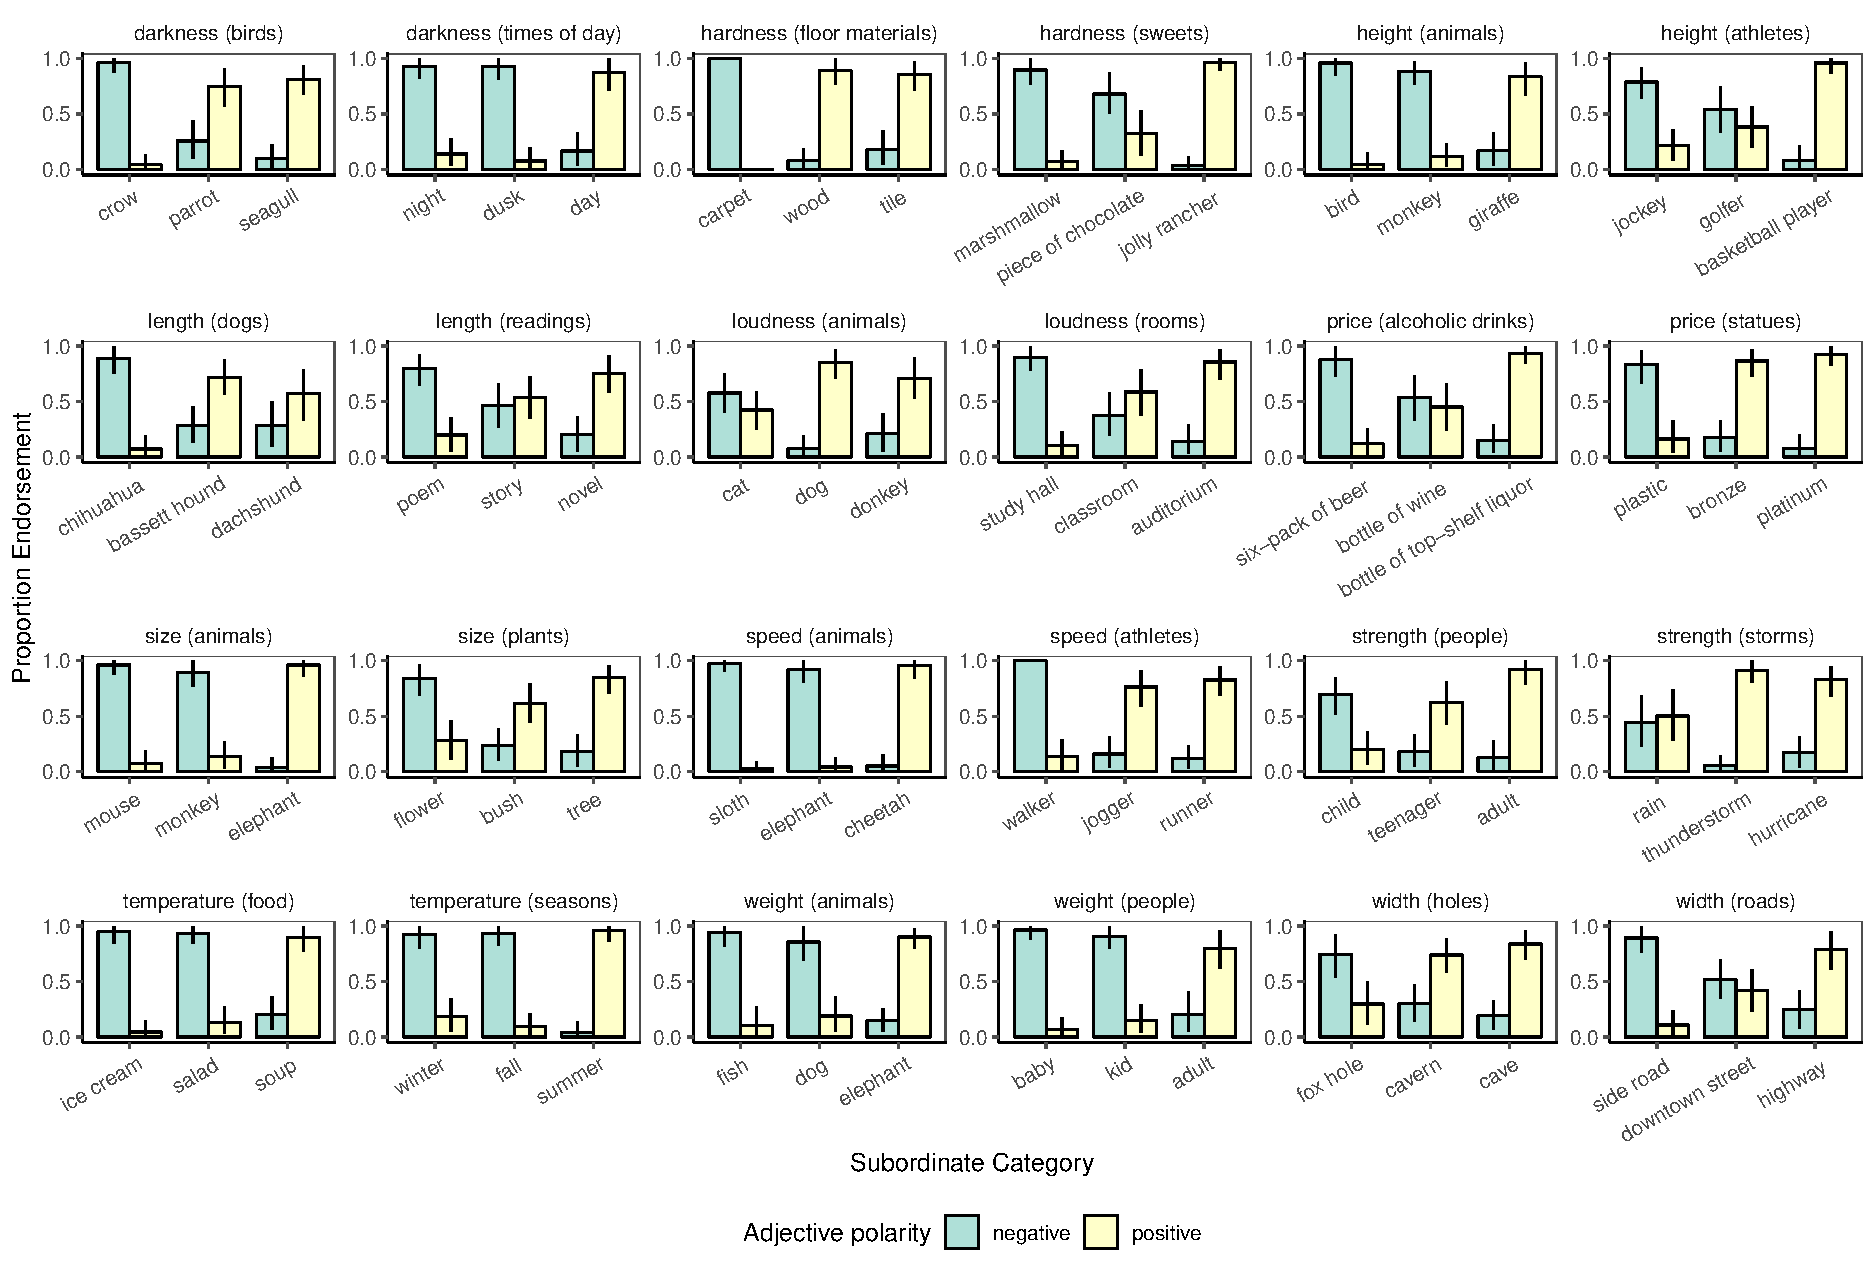
\includegraphics[width=\textwidth]{figs/bars_adj_finalExpt_pilot_byItem.pdf}
%{\centering 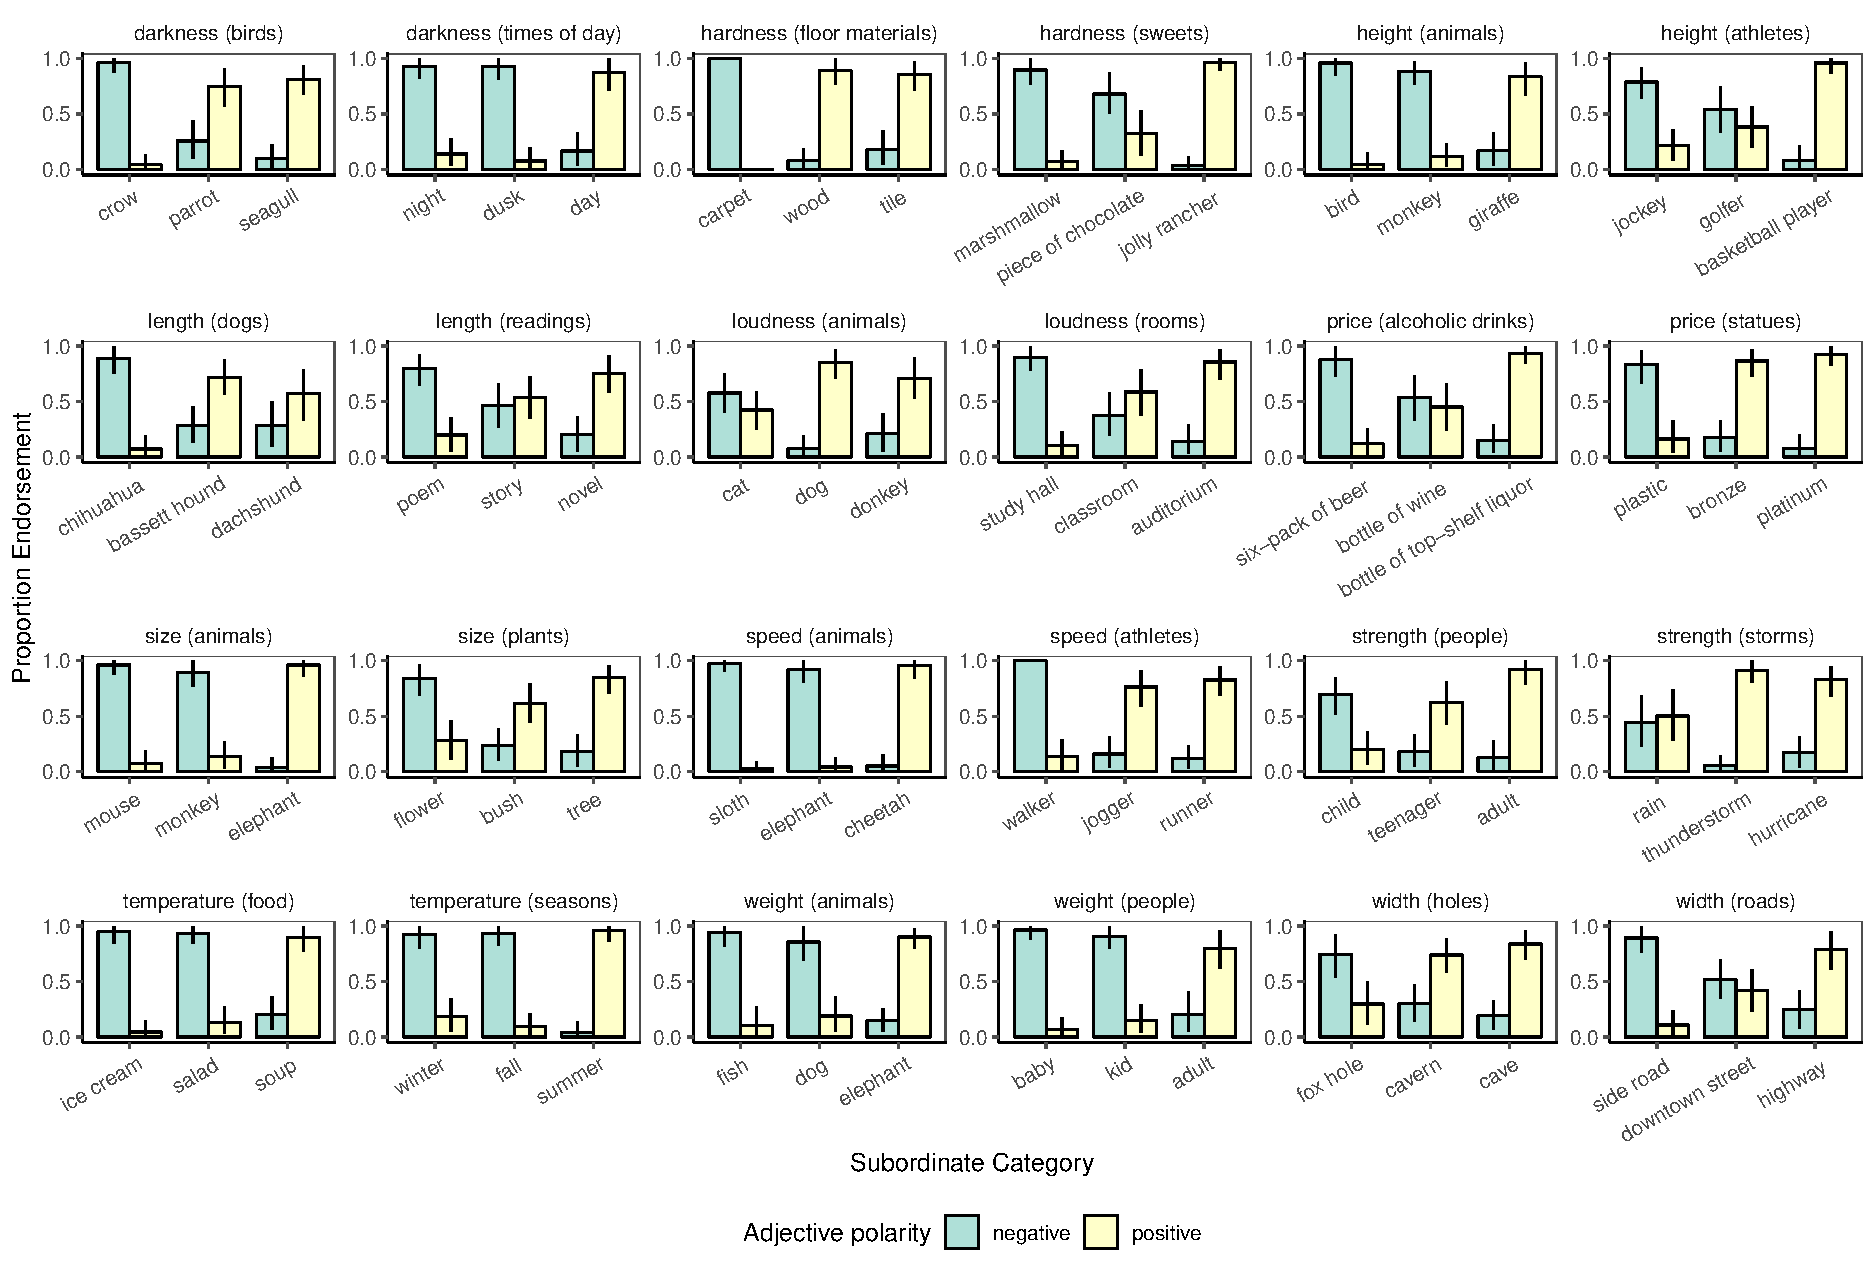
\includegraphics{figs/bars_adj_finalExpt_pilot_byItem} }
\caption{Experiment 2 results for a subset of the items.}\label{fig:adjEndorseItems}
\end{figure}

\subsection{Experiment 3: Comparison class inference}

Sample size, exclusion criteria, regression analysis, and cognitive model analysis were preregistered: \url{osf.io/XXXX}.

\subsubsection{Participants}

We recruited 1250 participants from Amazon's Mechanical Turk. 
This number was arrived at with the goal of collecting 50 comparison class paraphrases for each unique item in the data set.
Participants were restricted to those with U.S. IP addresses with at least a 95\% work approval rating.
In addition, participants were prohibited from participating in this experiment if they participated in Experiment 2.

\subsubsection{Procedure and Materials}

On each trial, participants were given a context sentence to introduce
the subordinate category (e.g., \emph{Tanya lives in Maryland and
steps outside in winter}). This was followed by an adjective sentence, which predicated either a positive- or negative-form gradable adjective over the item (e.g., \emph{Tanya says to her friend, ``It's warm.''}). Participants were asked \emph{What do you think Tanya meant?} and given a sentence frame they could complete with with a freely-produced comparison class:

\begin{quote}
It is warm relative to other \_\_\_\_\_\_.
\end{quote}

Materials were the same as in Experiment 2.
There were 756 unique trials. 
Each participant completed 30 trials. 
At the end of the task, participants were asked a memory check question where they had to select, from a list of 10 options, all of the items they could recall seeing. In the memory check, items were shown as adjective -- subordinate category pairs (``tall --- basketball player'') and the 5 distractors were either color or multidimensional adjectives paired with a category (e.g., ``green -- tennis ball''; ``beautiful -- painting'').




\begin{figure}[t!]
\centering
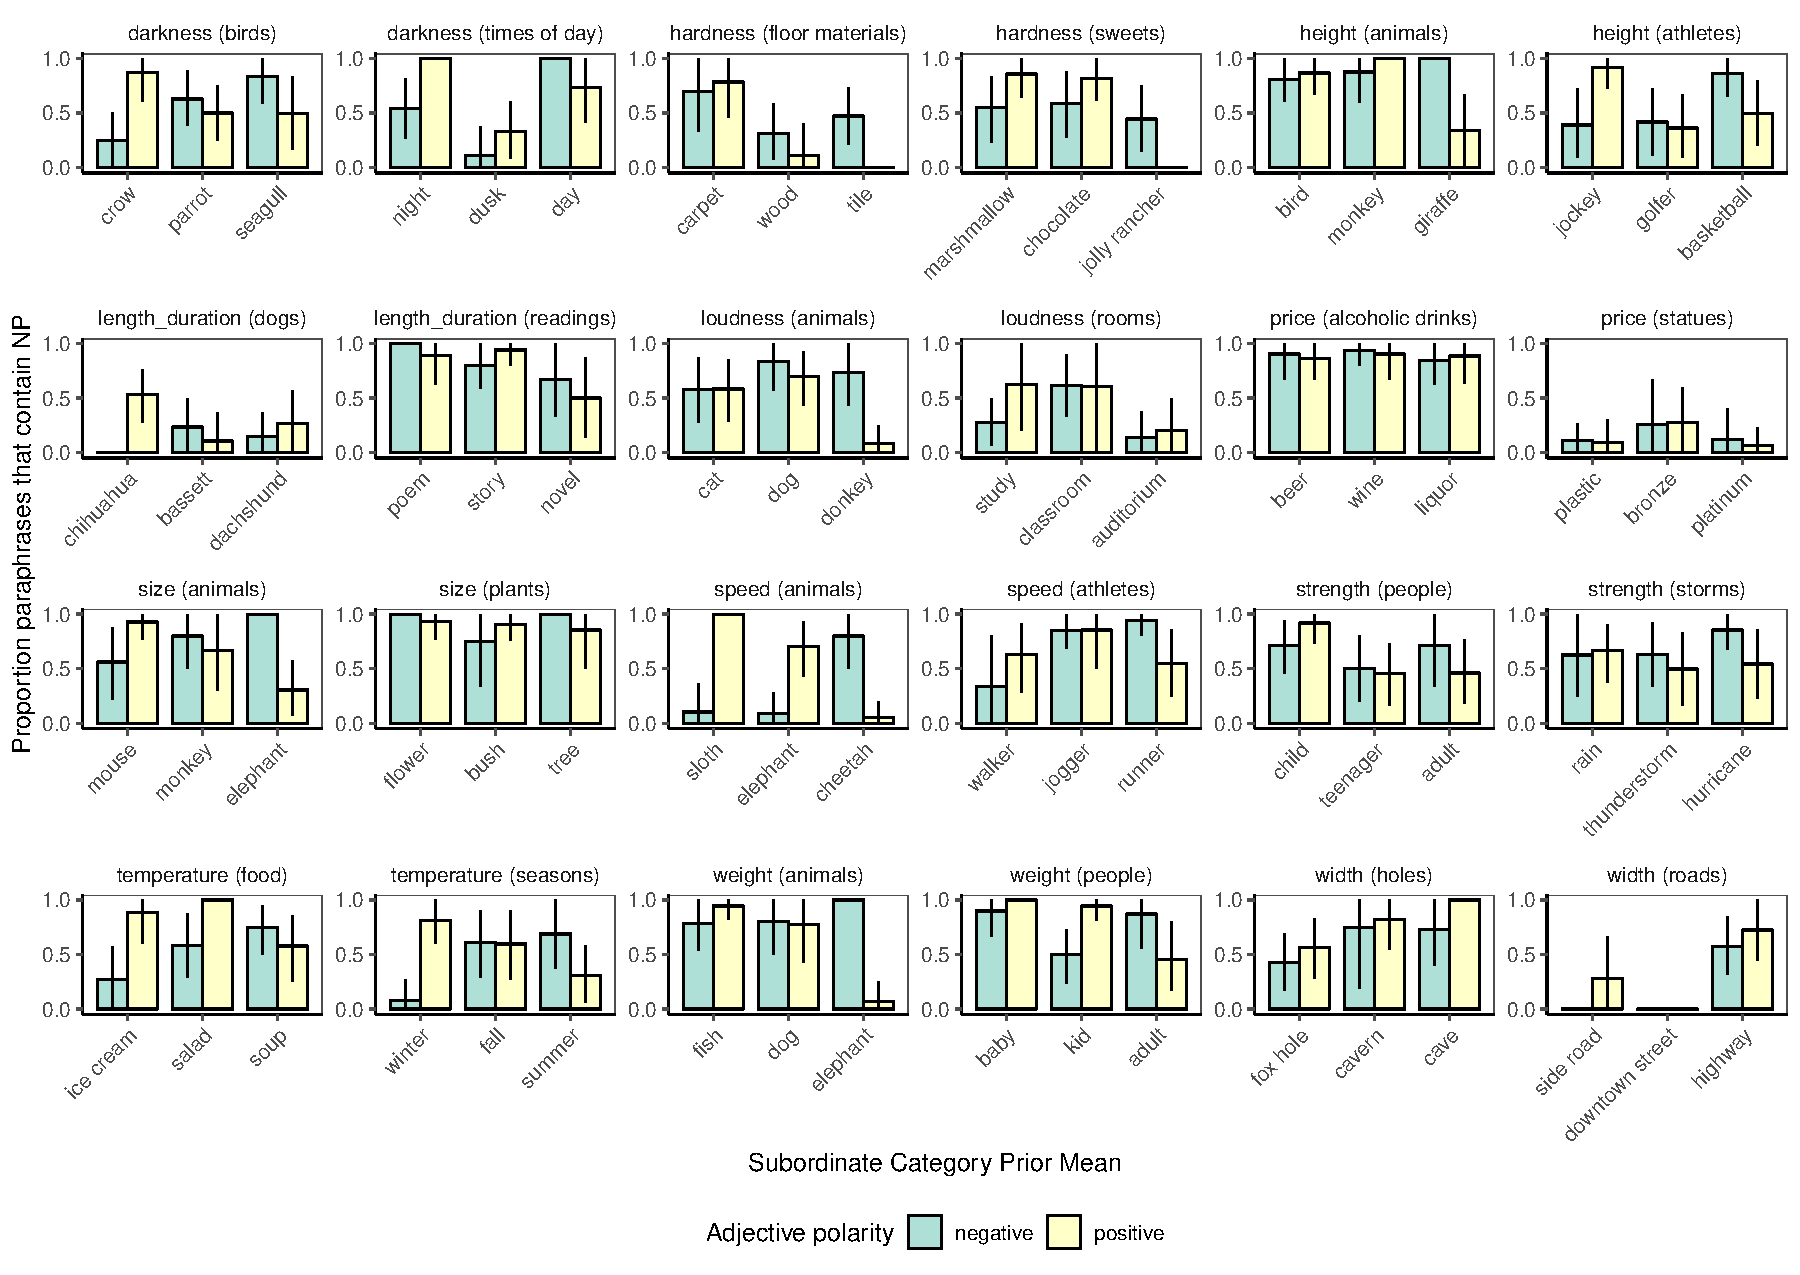
\includegraphics[width=\textwidth]{figs/bars_cc_finalExpt_pilot_byItem.pdf}
%{\centering 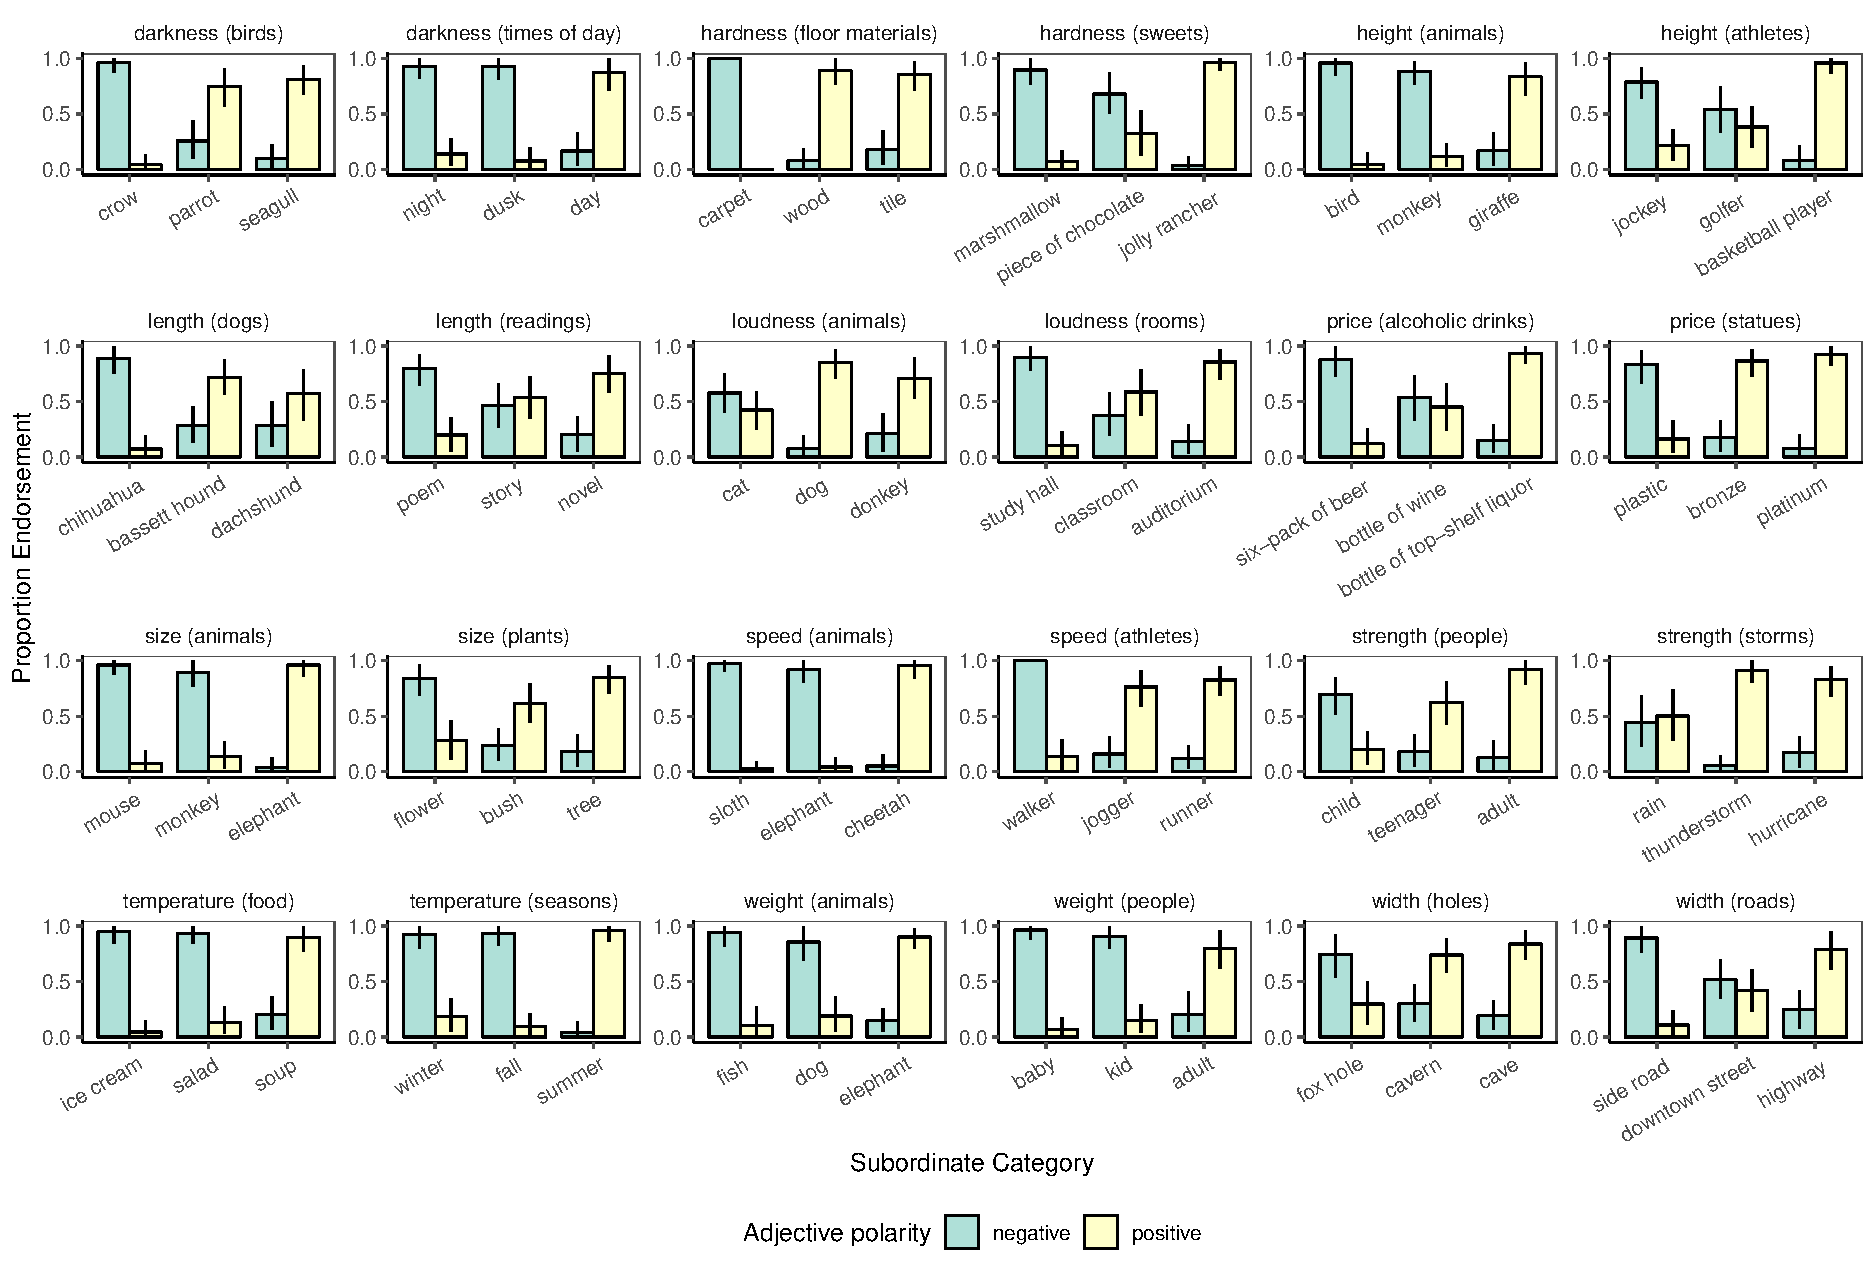
\includegraphics{figs/bars_adj_finalExpt_pilot_byItem} }
\caption{Experiment 3 results for a subset of the items.}\label{fig:ccInferenceItems}
\end{figure}

\subsubsection{Results}

Participants were excluded if they answered fewer than 7 out of 10 memory check questions accurately. 
Pilot testing suggested that participants primarily provide comparison class paraphrases that are identical to the subordinate class by which the referent is introduced (e.g., a basketball player) or a more general (basic or superordinate) category. 
Thus, we coded each response as either subordinate vs. basic/superordinate. 
\red{X responses were excluded because they could not be coded as either.}
%We observed no systematic differences between participants' responses when the superordinate category was previously mentioned in the context and those when it was not; thus, we collapse across these two conditions for all analyses. 
Figure XXX shows the proportion of participants choosing the \emph{subordinate} paraphrase for each item, revealing considerable variability both \emph{within}- and \emph{across}- scales. 
The predicted effects are visually apparent within each scale (compare with Figure XXX).
We build a logistic mixed-effects model to predict participants' subordinate class paraphrases; this model mirrors the structure of the model of Experiment 2 data.
We predict subordinate class paraphrases as a function of the general expectations about the subordinate category (low, medium, high; dummy coded with the medium category as the reference level), the adjective (positive vs. negative; difference coded), and their interaction; in addition, we include the maximal mixed effects structure by-item set and by-participant that mirrors this fixed effects structure.\footnote{
The model is subordinate\_inference $\sim$ gen\_expectations * adjective\_polarity + (1 + gen\_expectations * adjective\_polarity | participant) + (1 + gen\_expectations * adjective\_polarity | item\_set).
}

As predicted, the only regression coefficients that were credibly different from zero were the interaction terms. 
When the subordinate category was expected to be near the middle of the scale (e.g., a soccer player), there was not a credible difference between subordinate comparison classes for the positive form adjective (e.g., tall) and the negative form adjective (e.g., short): beta-weight and 95\% Bayesian credible interval: \brmresults{expt3_brm_pilot.csv}{adj_positiveness1}.
Also, there were no credible differences in comparison class inferences for the adjectives when the subordinate category was either near the high-end of the scale (e.g., basketball players; \brmresults{expt3_brm_pilot.csv}{np_positivenesspositive}) or the low-end of the scale (e.g., gymnasts; \brmresults{expt3_brm_pilot.csv}{np_positivenessnegative}).
When the subordinate category was expected to be near the high-end of the scale (e.g., the height of a basketball player), the positive form adjective (e.g., tall) led to credibly more inferences of a basic/superordinate comparison class than the negative form adjective (e.g., short) in comparison to middle-of-the-scale items (e.g., soccer player):  \brmresults{expt3_brm_pilot.csv}{np_positivenesspositive:adj_positiveness1}.
The opposite interaction term was also credibly different from zero: When the subordinate category was expected to be near the low-end of the scale (e.g., the height of a gymnast player),  hearing the positive form adjective led to credibly more inferences of a subordinate comparison class than hearing a negative form adjective in comparison to middle-of-the-scale subordinate categories:  \brmresults{expt3_brm_pilot.csv}{np_positivenessnegative:adj_positiveness1}.
This analysis confirms the primary hypothesis.

%Our qualitative predictions are confirmed using a generalized linear mixed effects model with main effects of adjective form (positive vs.~negative) and the \emph{a priori} judgment by the first author of whether the sub-category was expected to be low or high on the degree scale, and of critical theoretical interest, the interaction between these two variables. In addition, we included by-participant random effects of intercept and by-subordinate category random effects of intercept and interaction between form and strength\footnote{This was the maximal mixed-effects structure that converged.}. Confirming our two qualitative model predictions, there was an interaction between form and strength (\(\beta = -3.82\); \(SE = 0.57;\) \(z = -6.73\)) and there was an overall preference for subordinate category paraphrases (\(\beta = 1.23\); \(SE = 0.45;\) \(z = 2.70\)). The main effects of form and strength were not significant.
%
%We then test the simple effects. For items low on the degree scale (e.g., temperatures in winter), positive form adjectives were significantly more likely to imply subordinate comparison classes (\(\beta = 1.41\); \(SE = 0.15;\) \(z = 9.43\)), while the opposite is true for items high on the scale (e.g., summer days; \(\beta = -2.50\); \(SE = 0.19;\) \(z = -13.15\)). Participants reason pragmatically to resolve the comparison class, combining world knowledge with informativity as predicted by our model.

\subsection{Quantitative modeling}


The full model's posterior over the RSA and data-analytic parameters were consistent with prior literature and intuition. The maximum a-posteriori (MAP) estimate and 95\% highest probability density (HPD) intervals for model parameters specific to the \(L_1\) model used for comparison class inference were \(\alpha^{1}_{1} = 1.60 [1.10, 2.50]\), \(\beta = 0.13 [0.11, 0.19]\). Model parameters specific to the \(S_2\) model used for adjective endorsement: \(\alpha^{2}_{1} = 3.50 [0.60, 13.20]\), \(\alpha^{2}_{2} = 3.20 [2.60, 3.80]\). The inferred distributions corresponding to subordinate class priors were consistent with the \emph{a priori} ordering of these subordinate classes (low, medium, high) used in these tasks (Figure \ref{fig:modelParameters} top).

Finally, the full model's posterior predictive distribution does an excellent job at capturing the quantitative variability in comparison class inferences: \(r^2(30) = 0.96\), and adjective endorsements: \(r^2(30) = 0.98\) (Figure \ref{fig:posteriorPredictiveScatters}). Because of the overall preference for the subordinate comparison class, many of the data points are distributed above 0.5. Even for these fine-grained differences, the model does a good job at explaining the quantitative variability in participants' data (Figure \ref{fig:posteriorPredictiveScatters} right). Thus, the variability in comparison class inferences we observe in our behavioral data can be accounted for the constructs posited in our model (namely, the comparison class prior and degree priors).

\section{General Discussion}

%Inferring the comparison class from such a generative model goes beyond a model of concepts, however; listeners must reason about a speaker's behavior...


%
%
%This problem is closely tied to inferring the intended referent for an utterance (``Dogs are on my front lawn''? Ask Masoud for examples): When a listener determines 
%This omission is problematic for 
%
%
%
%
%Comparison classes are useful because they allow us to generalize the lexical semantics of many different kinds of adjectives or other \emph{relative} linguistic meanings. 
%Human cognition can use the minimal semantics with a flexible comparison class and create a multiplicity of interpreted meanings.
%
%Theories of semantic composition for dealing with relative adjectives assume some comparison class.
%
%
%

%understand that \emph{big} is relative \cite{Sera1987} and that the
%comparison class can change





%Previous research has focused on what occurs during language understanding once a comparison class is determined.
%The question of how listeners decide upon a comparison class when it is not stated explicitly (e.g., ``It's warm relative to other days this winter'') has been addressed neither formally nor empirically.


%The speaker's choice of noun phrase can strongly influence the comparison class  (e.g.,  a \emph{big snowman} is probably big relative to other snowmen), though it need not determine it: saying ``That's a big snowman'' to a 4-year-old might mean \emph{big relative to snowmen a 4-year-old could build} \cite{kamp1975two}. 
 
% In this paper, we investigate the first aspect of this open-ended inference problem, deciding among multiple possible comparison classes. 


%The existence of comparison classes for understanding relative adjectives is uncontroversial \cite{cresswell1976semantics, klein1980semantics, kennedy2005scale, bale2008universal, Bale2011, Solt2009}. %\red{more standard citations for this?}

Interpreting language requires understanding the context in which the words are uttered.
Yet, the context is almost never described explicitly but left to the listener to pragmatically reconstruct. 
Inferring comparison classes for scalar adjectives (e.g., \emph{tall}) is thus a case study in the larger phenomenon of the pragmatic reconstruction of context. 
In this paper, we find that listeners flexibly adjust the comparison class in systematic ways, which we elicit in an open-ended response measure.

We introduced a minimal extension to an adjective interpretation Rational Speech Act model to account for these flexible inferences.
% it to flexibly reason about the implicit comparison class (e.g., \emph{tall for a person}~vs.~\emph{tall for a basketball player}).
This model made the qualitative prediction that listeners should prefer more specific (e.g., subordinate-level) comparison classes when the adjective conflicts with their general expectations about a member of a category (e.g., a basketball player who is short), and we showed how this inference requires pragmatic reasoning, which a literal interpretation model cannot draw. 
The model also made quantitative predictions about the gradability of this inference given knowledge about properties and categories. 
The strong quantitative fit of this model to the free-production data provides compelling evidence that the comparison class inference can be viewed as a Bayesian inference operating on top of a pragmatic language understanding architecture. 

In addition to the novel empirical data and the computational model of comparison class inference, this paper also presents experimental and data-analytic methodological innovations. 
On the experimental side, we articulated an explicit generative model of our items, which we deployed on human participants to construct a large and diverse set of linguistic stimuli (n = 756 unique stimuli). 
While this procedure was not entirely ``end-to-end'' (i.e., we authors still needed to curate, edit, and add context to the items), the method presents a significant advance beyond the traditional method of the scientist constructing a small set of stimuli, often inadvertently optimized to test a theory \cite<cf.,>{Clark1973}.
On the data-analytic side, we coupled a \emph{descriptive Bayesian} approach \cite{tauber2017} with the productivity of probabilistic models of language understanding \cite{Goodman2016, scontras2017probabilistic} to jointly model two complementary language tasks and infer the relevant prior knowledge that is shared between the tasks.
The major feature of this method is that it allows us to back-out quantitatively detailed domain knowledge that would be otherwise inaccessible through traditional prior elicitation techniques because human participants lack requisite knowledge of the quantitative scales (e.g., how many decibels is the sound of a rooster's crow?); in addition, this method has the feature that  participants respond only to simple, natural language questions rather than estimate numerical quantities for which complicated linking functions must be designed \cite<cf.,>{Franke2016}. 
The fully Bayesian language approach we pioneer here also provides further constraints on the language understanding models, which must predict quantitative data from two similar but distinct language experiments. 
The productivity of natural language can thus be harnessed to productively design experiments that further constrain and test computational models of language and cognition.

Our work builds on previous experimental work on adjective understanding.
\citeA{Barner2008} found that 4-year-olds use the noun to constrain the comparison class (e.g., the comparison class for a ``tall pimwit'' is \emph{other pimwits} and does not include other non-pimwit objects).
\citeA{Ebeling1994} showed how even younger children can flexibly shift between qualitatively different kinds of comparison classes (e.g., big \emph{for a mitten} vs. big \emph{relative to the objects around it}).
Our work builds upon these previous studies by showing how the comparison class can shift as well as providing a general purpose computational solution to this open-ended inference problem.

%It's been suggested that there exist qualitatively different kinds of
%comparison classes, constructed by reference to either: the perceptual
%context (a \emph{perceptual comparison class}), a goal of an agent or
%intended use of an object (a \emph{functional comparison class}), and
%the kind of the referent (a \emph{conceptual comparison class}; Ebeling
%\& Gelman, 1994). In this paper, we investigated the latter, but the
%question remains about how a listener should decide to switch between
%different kinds of comparison classes. For example, if Ann and Carl are
%deciding what to do on a Friday night, Carl suggest the ballet, to which Ann replies ``The
%ballet is expensive'', Carl should understand Ann's statement relative
% \emph{other ways they could spend their Friday night}, a kind-of
%functional comparison class. Goal inference is thus an associated
%ingredient in comparison class inference, and integrating the two
%should be a target for future work.

A relevant detail of our experiment contexts is that the speaker's sentence did not include a noun phrase to describe the referent (i.e, the speaker said ``He is tall'' as opposed to ``That basketball player is tall''). 
We found that when the adjective is consistent with the listener's general expectations about the category (e.g., the basketball player is tall), listeners prefer comparison classes that are also more general (i.e., tall for a person). 
Intuitively, the speaker's intentional production of a noun phrase could more directly communicate the comparison class by revealing how the speaker is conceptualizing the referent (e.g., \emph{the speaker is conceiving of this person as a basketball player}).
The extent to which this inference holds could also depend upon the syntactic structure of the sentences: 
Prenominal uses of the adjective (e.g., ``He's a tall basketball player'') might be an even stronger cue. 
Indeed, prenominal uses are argued to be ideal for a child learning the meaning of novel adjectives \cite{Waxman2001, Mintz2002, Sandhofer2007} perhaps because it is such a strong cue to the comparison class.
Future work should investigate the interaction between syntactic structure and pragmatic inferences regarding the comparison class.

We observe in our quantitative modeling results that a uniform prior distribution over the specific~vs.~general comparison classes is unlikely (Figure \ref{fig:modelParameters} bottom). 
%For example, the comparison class of ``people'' for heights of individuals is relatively more salient than the class of ``produce'' (or, ``fruits and vegetables'') for the weights of particular fruits and vegetables. 
As a proxy for the prior probability of a comparison class, we used a (logistic) linear function with an intercept to reflect a basic-level bias \cite{rosch1975family} and a slope of the frequency of the noun phrase in a corpus. 
Corpus frequency is a composite measurement of factors relevant for speech production. 
Its utility in this model suggests that utterances without an explicit comparison class (e.g., ``It's warm outside'') may in fact be incomplete sentences, in a way analogous to sentence fragments studied in noisy-channel models of production and comprehension \cite{bergen2015strategic}. 

The phenomenon of comparison class inference is a case study in inferring context, or deciding upon what is in common ground between speaker and listener.
The situation we model is one of asymmetric knowledge: The listener is uncertain about the relevant context, but the speaker does not represent the listener's uncertainty. 
Were the speaker to accurately represent this uncertainty in the listener, then the speaker would have produced a more circumscribed utterance (e.g., by articulating the comparison class with a \emph{for} phrase).
%The comparison class assumed by the speaker, then, acts as a kind of presupposition, and for the formal modeling mechanism we employ has in fact been deployed in modeling presuppositions \cite<e.g., ``When did John quit smoking?'' implies that John used to smoke;>{Qing2016projective}.
In our experiment, the speaker is talking to a third party and the actual comparison class inference may be a result of the participants' uncertainty about the information in common ground between the interlocutors; future work should examine dyadic interactions to better understand the role of asymmetric knowledge in inferring comparison class.
%comparison class most likely to make the utterance true while
%prioritizing more specific (lower variance) classes because they are
%more informative. It also made quantitative predictions about how
%background knowledge about the degree scale and what classes are likely
%to be talked about \emph{a priori} should inform this inference in a
%graded fashion. Both qualitative predictions of the model were borne out
%in our behavioral experiment, and the quantitative predictions were
%confirmed using a novel data analytic technique.


%Investigations of how human listeners understand vague adjectives have
%shed light on the precise mechanisms by which people interpret
%context-sensitive language, but have had little to say about how
%listeners decide upon what counts as the appropriate context. In this
%paper, we take the first step towards investigating the flexibility in
%the class against which an entity can be implicitly compared, a very
%basic form of context. Resolving underspecification by means of a comparison is not unique to
%\emph{gradable adjectives} like ``big'' or ``tall'', but is
%a general problem for language understanding. ``John ate \emph{a
%lot} of hot dogs'' probably means four or five hot dogs, whereas
%``John ate \emph{a lot} of potato chips'' could imply a quantity
%over a hundred (Schöller \& Franke, 2017); ``Robins lay eggs''
%means roughly that \emph{female robins} lay eggs, whereas
%``Robins fly'' entails something stronger, most or all robins fly
%({\textbf{???}}; {\textbf{???}}). Even noun concepts (e.g.,
%``furniture'') are graded (Rosch \& Mervis, 1975) and can be made
%more precise in context. Investigating how listeners interpret words
%like ``big'' is thus a case study of a crucial, general problem in
%language understanding: Understanding context-sensitive language.
%
%We investigated the question of how a listener decides among multiple
%possible conceptually-based comparison classes (e.g., tall for a
%basketball player vs.~tall for a person). It is notable that our model
%was able to account for inferences about items that did not fall into
%strict hierachies (e.g., \emph{movies} is not subordinate to
%\emph{things you watch online}) as well as items that did (e.g.,
%basketball players and people). This result suggests that our modeling
%framework can easily extend into cross-cutting comparison classes (e.g.,
%\emph{men}, \emph{people of a certain age}, \emph{basketball players}).
%
%\subsection{The phenomenon of comparison class
%inference}

%\subsection{Comparison class prior}
%
%We observe in our quantitative modeling results that a uniform prior
%distribution over the experimentally supplied comparison class
%alternatives is unlikely (Figure \ref{fig:modelParameters} bottom). For
%example, the comparison class of ``people'' for heights of
%individuals is relatively more salient than the class of
%``produce'' (or, ``fruits and vegetables'') for the weights
%of particular fruits and vegetables. We used the frequency of the class
%in a corpus as a proxy for their prior probability \(P(c)\), which was
%sufficient to account for differences in baseline class probability both
%\emph{between}- and \emph{within}-scales.
%
%Corpus frequency is a composite measurement of factors relevant for
%speech production. Its utility in this model suggests that utterances
%without an explicit comparison class (e.g., ``It's warm outside'')
%may in fact be incomplete sentences, in a way analogous to sentence
%fragments studied in noisy-channel models of production and
%comprehension (Bergen \& Goodman, 2015). Another (non-mutually
%exclusive) possibility is that the comparison class prior reflects
%basic-level effects in categorization (Rosch \& Mervis, 1975). Future
%work should attempt to understand these factors to construct a more
%complete theory of the comparison class prior.
%


\section{Conclusion}

The words we say are often too vague to have a single, precise meaning,
and only make sense in context. The context, however, can also be
underspecified, leaving the listener in the dark about both the
speaker's intended meaning and about the context through which the
listener is to make sense of the conversation. This work suggests that listeners infer a lot from a little:
The meaning and the context from a single vague utterance.


\section{Acknowledgements}

This work was supported in part by NSF Graduate Research Fellowship
DGE-114747 to MHT and a
Sloan Research Fellowship, ONR grant N00014-13-1-0788, and DARPA grant
FA8750-14-2-0009 to NDG.

\newpage


\bibliographystyle{apacite}

%\setlength{\bibleftmargin}{.125in}
%\setlength{\bibindent}{-\bibleftmargin}

\bibliography{comparison-class}

%\newpage
%\section{Appendix}
%
%
%%Gradable adjectives like \emph{warm} and \emph{cold} are vague
%%descriptions of an underlying quantitative scale (e.g., temperature).
%Classic semantic theories posit the meaning of gradable adjectives to simply be that the scalar degree $x$ (e.g., temperature) is greater than or less than a contextually-supplied standard of comparison  \(\theta_c\): \([\![u_{pos}]\!] = x > \theta_c\), for positive-form adjectival utterance \(u_{pos}\) (e.g., warm) and \([\![u_{neg}]\!] = x < \theta_c\), for negative-form adjectival utterance \(u_{neg}\) (e.g., cold).
% Lassiter \& Goodman (2013) model the context-sensitivity of these adjectival utterances using threshold semantics, where
%the threshold is probabilistically set with respect to a comparison class \(c\) via pragmatic reasoning :
%
%\begin{align}
%L_{1}(x, \theta \mid u, c) &\propto S_{1}(u \mid x, \theta) \cdot P(x \mid c) \cdot P(\theta) \label{eq:L1} \\
%S_{1}(u \mid x, \theta, c) &\propto \exp{(\alpha_1 \cdot (\ln {L_{0}(x \mid u, \theta, c)} - \text{cost}(u)))} \label{eq:S1}\\
%L_{0}(x \mid u, \theta, c) &\propto {\delta_{[\![u]\!](x, \theta)} \cdot P(x \mid c)} \label{eq:L0}
%\end{align}
%
%Eqs. \ref{eq:L1} - \ref{eq:L0} are the Rational Speech Act mode  Lassiter \& Goodman (2013). 
%In this model, a pragmatic listener \(L_1\)
%tries to resolve the degree \(x\) (e.g., the temperature)
%from the adjectival utterance she heard \(u\) (e.g., ``it's warm''), by assuming the utterance came from an approximately rational Bayesian
%speaker \(S_1\) trying to inform a naive listener \(L_0\), who in turn
%updates their prior beliefs \(P_c(x)\) via an utterance's literal meaning
%\([\![u]\!](x, \theta)\).
%Formally, the literal meaning is represented by the
%Kronecker delta function \(\delta_{\mbox{ $[\![ u ]\!]$}(x, \theta)}\)
%that returns probabilities proportional to \(1\) when the utterance is
%true (i.e., when \(x > \theta\)) and \(0\) otherwise.
%The key innovation used for modeling gradable adjectives is to have uncertainty over the
%semantic variable---the threshold \(\theta\) (Eq. \ref{eq:L1}). In
%Lassiter and Goodman (2013)'s model, \(\theta\) comes from an improper uniform
%prior distribution over thresholds defined over the real numbers and is resolved by the
%listener reasoning about the different thresholds a speaker might be
%using \(S_{1}(u \mid x, \theta)\) as well as the probabilities of
%different states of the world \(P(x \mid c)\) (e.g., different
%temperatures). Assuming the adjective adds some cost to the speaker's
%utterance (Eq. \ref{eq:S1}), the meaning of a gradable adjectives (e.g.,
%``warm'') is resolved by the pragmatic listener to mean something
%like ``significantly greater temperature than one might expect''
%(Lassiter \& Goodman, 2015). Critically, what ``one might
%expect''---the prior distribution over temperatures \(P(x \mid c)\)---is
%always with respect to some comparison class \(c\) (Eqs. \ref{eq:L1} \&
%\ref{eq:L0})
%

\end{document}
